\chapter{Application of Modeling}\label{sec:dem-studies}

This chapter demonstrates the usefulness of the numerical tools introduced in \cref{ch:modeling-development} in probing inter-particle contact information, pebble bed heat transfer, and bed morphology changes altering thermophysical properties. The DEM, CFD-DEM, and DEM-LBM tools are put to work examining representative volumes of pebble beds of ceramic breeders from fusion reactors. In almost all cases, the pebble bed volumes accommodate approximately \num{10000} pebbles. Typically, the bed is confined in one direction by two primitive, rigid walls that also are constant temperature boundaries to act as heat sinks. I also employ periodic boundary conditions to represent an infinite length in the given direction. The third direction is often in the gravity direction for which we have an adiabatic, primitve, and rigid roof and ceiling.

The first study considers the heat transfer in a pebble bed purely through contact conduction of grains in the ensemble. In this pebble bed, I employ DEM tools to apply a nuclear heating source and allow the bed to reach a thermal steady-state with the cooling walls. In such a way, an effective thermal conductivity of the bed is determinable. I then induce a fictitious pebble damaging method to the bed and check the changes to effective thermal conductivity. The DEM tools are used to then interrogate many micromechanical interactions in the pebble bed which we use to deduce the source of changes to the effective thermal conductivity.

In the second study, the same pebble bed is analyzed but this time the helium purge gas is included via the coupled CFD-DEM tools. I again induce some fictitious damage to the pebble bed and monitor changes to the thermophysical properties and their relationship to the cases when the helium purge gas was neglected. The study reveals important features of the helium influence on heat transfer in the bed.

In the third study, I take snapshots of two beds (a standard bed and a damaged one) and load them into LBM models. With lattice-Boltzmann it is possible to analyze the tortuous path of helium moving through the pebble bed and discover interesting features of the purge gas thermal interaction that was masked by the simplifications of the volume-average approach of CFD-DEM.


























\section{Temperature Distributions with Breeder Orientation, Pebble Fragmentation}\label{sec:isfnt-12}


\subsection{Introduction}

We apply coupled computational fluid dynamics and discrete element method (CFD-DEM) modeling tools with new numerical implementations of pebble fragmentation to study the combined effects of granular crushing and ensemble restructuring, granular fragment size, and initial packing for different breeder volume configurations. In typical solid breeder modules, heat removal from beds relies on maintaining pebble-pebble and pebble-wall contact integrity. However, contact is disrupted when an ensemble responds to individually-crushed pebbles. Furthermore, restructuring of metastable packings after crushing events are, in part, dependent on gravity forces acting upon the pebbles. We investigate two representative pebble bed configurations under constant volumetric heat sources; modeling heat removed from beds via inter-particle conduction, purge gas convection, and contact between pebble beds and containers. In one configuration, heat is removed from at walls oriented parallel to the gravity vector (no gap formation possible); in the second, heat is removed at walls perpendicular to gravity, allowing for the possibility of gap formation between bed and wall. Judging beds on increase in maximum temperatures as a function of crushed pebble amount, we find that both pebble bed configurations to have advantageous features that manifest at different stages of pebble crushing. However, all configurations benefit from achieving high initial packing fractions.



\subsubsection{Simulation domain, boundary conditions, and material properties}

Two ITER-relevant volumes are considered in this study, sketched in \Cref{fig:x-domain,fig:y-domain}. They are differentiated from each other by gravity's direction in the configuration. Because of their similarity, we use generic coordinate systems $(\chi, \zeta)$. Thus $\chi$-configurations, shown in \Cref{fig:x-domain}, have $\chi = y$ and $\zeta = x$ while $\zeta$-configurations, \Cref{fig:y-domain}, have $\chi = x$ and $\zeta = y$. The $\zeta$-configuration in this study is meant to represent the orientation of European Union's TBM \cite{Hernandez2013}, while the $\chi$ configuration is an orientation adopted by many other current TBM designs in ITER \cite{Cho2008,Feng2012a}.

\begin{figure}[!ht]
    \centering
    \begin{subfigure}[b]{0.44\textwidth}
        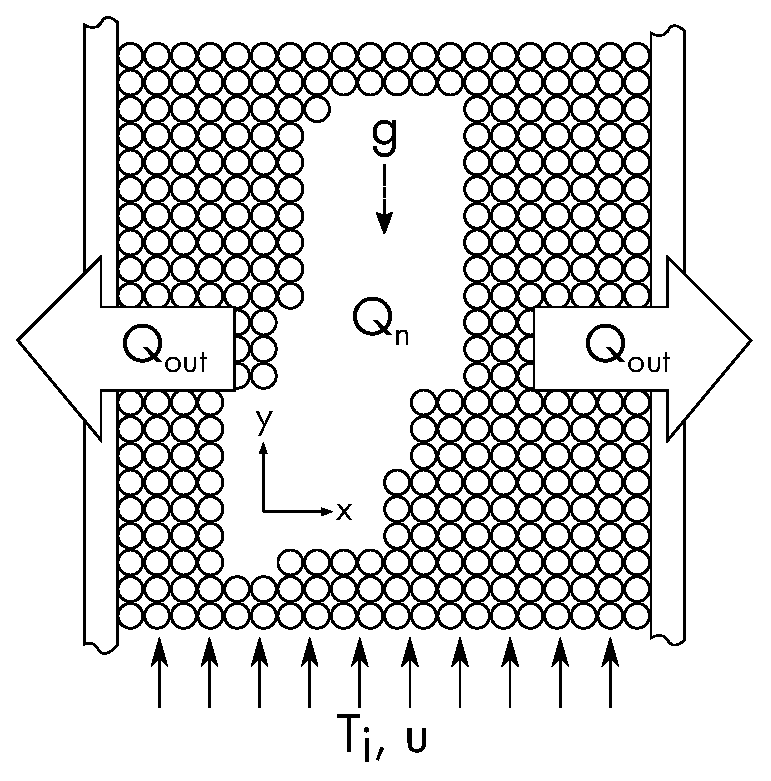
\includegraphics[width = \textwidth]{figures/x-domain.eps}
        \caption{$\chi$-configuration: heat removed in the $x$-direction.}\label{fig:x-domain}
    \end{subfigure}
    ~
    \begin{subfigure}[b]{0.44\textwidth}
        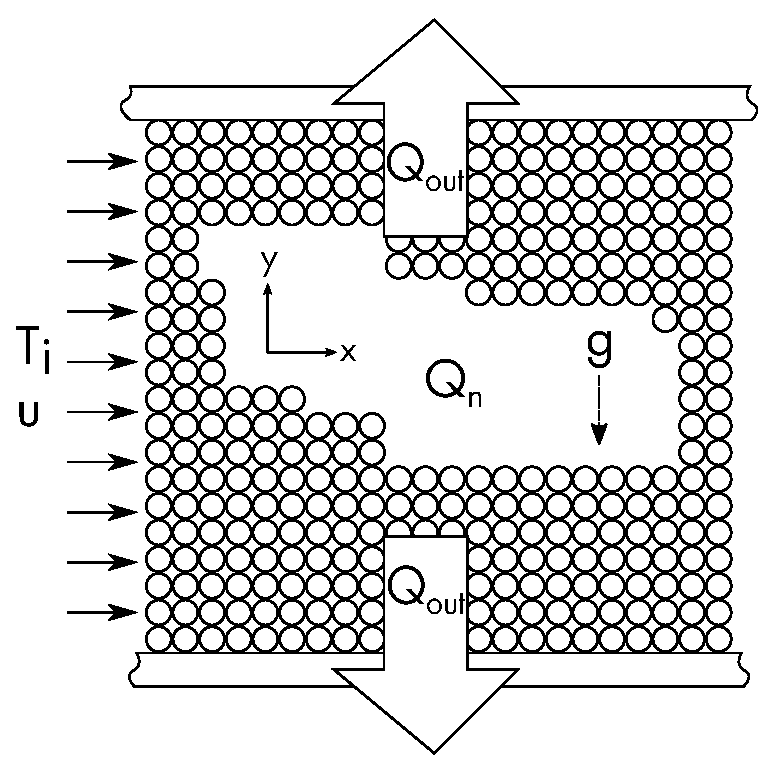
\includegraphics[width = \textwidth]{figures/y-domain.eps}
        \caption{$\zeta$-configuration: heat removed in the $y$-direction}\label{fig:y-domain}
    \end{subfigure}
    \caption{Sketches of the two breeder orientations show that gravity settling will not allow gaps between pebbles and walls in the $\chi$-configuration. However for the $\zeta$-configuration, gravity-induced resettling can create a gap between pebbles and upper wall. }\label{fig:domains}
\end{figure}

In terms of the generic coordinates, outflow of bed heat to coolant is along $\zeta$. Constant temperature boundaries, $T_w$, exist at the edges of that dimension. As sketched in \Cref{fig:domains}, gravity resettling in the $\chi$ configuration will not allow gap formation between bed and wall. However, in the $\zeta$-config it is possible for a gap to form between top coolant walls and pebbles after gravity resettling. A constant nuclear heat rate was applied to every particle in the bed which is representative of the highest source term anticipated in current ITER designs of solid breeder blankets, $q''' = $~\SI{8e6}{\watt\per\meter\cubed}.

The simulation consists of pebbles of diameter $d_p = $~\SI{1}{\milli\meter}, in beds filled to two initial packing fractions, $\phi_{1,2} = 62, 64\%$. Mechanical properties of the pebbles are given in \Cref{tab:peb-props}. To note is the Young's modulus chosen for pebbles in this study. In a past experimental study, Van Lew \textit{et al}. found that individual pebbles behaved in a manner indicative of having a Young's modulus from 20 to 60\% of values reported in literature for sintered blocks of \lit~and \lis~\cite{VanLew2015a}. Therefore to maintain some generality to this study, we have chosen a Young's modulus at a nominal value of $E=$~\SI{60}{\giga\pascal} to generically represent either ceramic pebble.

Pebble bed widths in $\zeta$ are \SI{20}{\milli\meter}, a size comparable to breeding volumes of many ITER TBM designs \cite{Hernandez2013,Cho2008,Feng2012a}. Bed depths (in the $z$-direction, in/out of the page in \Cref{fig:x-domain,fig:y-domain}) are \SI{5}{\milli\meter}, with periodic boundary conditions. Bed lengths in $\chi$ vary to accommodate \SI{6000} pebbles, initially, with given initial packing fractions; the length is approximately \SI{50}{\milli\meter}. Virtual walls are placed at extents of $\chi$ and $\zeta$ dimensions. Walls in $\zeta$ had constant temperature boundaries of $T_{w,s}$, all walls have mechanical and thermal properties of structural steel, given in \Cref{tab:wall-props}.

Fluid domains, overlaid on DEM pebbles, have fluid inlet and outlet regions of lengths \SI{10}{\milli\meter} and approximately \SI{51}{\milli\meter}, respectively. The side walls of the fluid domain were adiabatic in inlet and outlet regions and had constant temperature boundaries where they contacted the pebble bed, $T_{w,f}$. Fluid entered with a constant velocity magnitude of \SI{5}{\centi\meter\per\second} and constant temperature $T_i$. At present, temperature-dependencies of helium properties have not been incorporated into the model. Over the range of \SIrange{400}{900}{\celsius}, increases in helium momentum and thermal diffusivities are both essentially linear and thus an arithmetic mean for properties over that range is used as a first approximation. Future models will incorporate temperature-dependence of fluid properties. Fluid transport properties are given in \Cref{tab:fluid-props}. 
%---------------------------------------------------------------------------------------
% FIGURES
%---------------------------------------------------------------------------------------
% \begin{figure*}[!ht]
%        \centering
%        \begin{subfigure}[b]{0.45\textwidth}
%                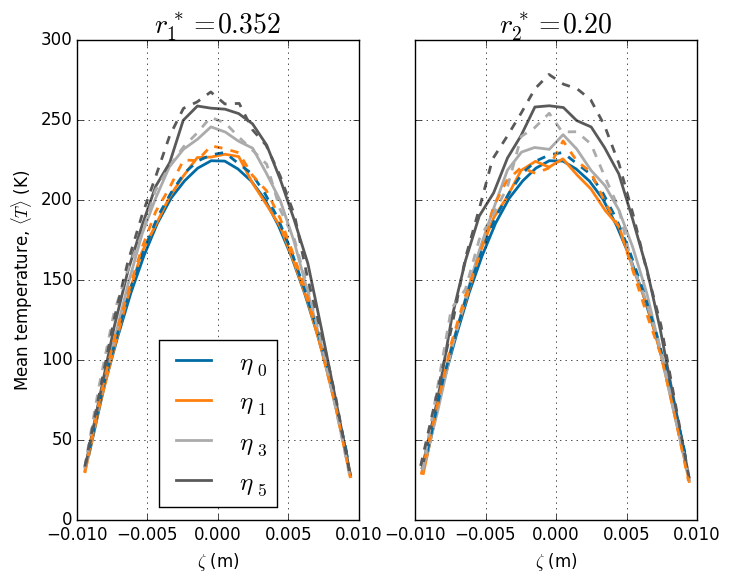
\includegraphics[width=\textwidth]{figures/62-percent-T-profiles.png}
%                \caption{Initial packing fraction of $\phi_1 = 0.62$.}
%                \label{fig:62-T-profile}
%        \end{subfigure}%
%        ~ %add desired spacing between images, e. g. ~, \quad, \qquad, \hfill etc.
%          %(or a blank line to force the subfigure onto a new line)
%        \begin{subfigure}[b]{0.45\textwidth}
%                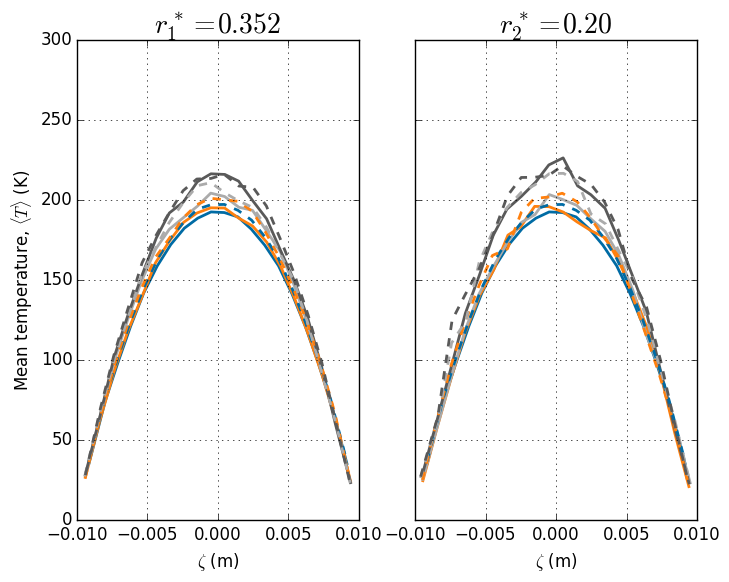
\includegraphics[width=\textwidth]{figures/64-percent-T-profiles.png}
%                \caption{Initial packing fraction of $\phi_2 = 0.64$.}
%                \label{fig:64-T-profile}
%        \end{subfigure}
%        \caption{Solid lines are cases where gravity is in the $\chi$ direction, dashed lines for gravity in the $\zeta$ direction; color is by percent of crushed pebbles, $\eta$.}
% \label{fig:T-profiles}
% \end{figure*}


%---------------------------------------------------------------------------------------
% TABLES
%---------------------------------------------------------------------------------------
\begin{table}[ht]
\centering
\caption{Mechanical and thermal properties of ceramic pebbles in the DEM domain. Aside from $E_s$, properties come from \cite{Gierszewski1998} with $\epsilon = 0.2$}
\label{tab:peb-props}
\resizebox{0.45\textwidth}{!}{%
\begin{tabular}{@{}lcS[table-format=3.2]@{}}
\toprule
%properties are coming from the lit_props.py file in the thesis scripts folder. Double check if you want
Property                                           & Symbol    & \text{Value} \\ \midrule
Young's modulus (\si{\giga\pascal})                & $E_s$     & 60.    \\
Poisson ratio                                      & $\nu_s$     & 0.24  \\
thermal conductivity (\si{\watt\per\meter\per\kelvin}) & $k_s$     & 1.79   \\
diameter (\si{\meter})                             & $d_p$     & 0.001     \\
pebble-pebble friction coefficient                 & $\mu_s$   & 0.2   \\
pebble-wall friction coefficient                   & $\mu_w$   & 0.2   \\ 
heat capacity (\si{\joule\per\kilo\gram\per\kelvin})   & $c_{s}$     & \num{1.45e3}  \\
thermal expansion coefficient (\si{\per\kelvin})   & $\beta_s$ & \num{1.77e-5}      \\
density (\si{\kilo\gram\per\cubic\meter})          & $\rho_s$  & \num{3.44e3}  \\ \bottomrule
\end{tabular}}
\end{table}

\begin{table}[ht]
\centering
\caption{Mechanical and thermal properties and boundary conditions of structural container in the DEM domain \cite{Fokkens2003}.}
\label{tab:wall-props}
\resizebox{0.45\textwidth}{!}{%
\begin{tabular}{@{}lcS[table-format=3.2]@{}}
\toprule
Property                                           & Symbol    & \text{Value} \\ \midrule
Young's modulus (\si{\giga\pascal})                & $E_w$     & 175.    \\
Poisson ratio                                      & $\nu_w$     & 0.30  \\
thermal conductivity (\si{\watt\per\meter\per\kelvin}) & $k_w$     & 29.0   \\ 
wall temperature (\si{\kelvin})                     & $T_{w,s}$        & 573    \\ \bottomrule
\end{tabular}}
\end{table}

\begin{table}[ht]
\centering
\caption{Transport properties of helium and boundary conditions in the CFD domain; mean values over the temperature range \SIrange{400}{900}{\celsius}.}
\label{tab:fluid-props}
\resizebox{0.45\textwidth}{!}{%
\begin{tabular}{@{}lcl@{}}
\toprule
% properties in excel sheet in thesis scripts folder
Property                                           & Symbol    & \text{Value} \\ \midrule
thermal conductivity (\si{\watt\per\meter\per\kelvin}) & $k_f$     & \num{3.40e-1}   \\
heat capacity (\si{\joule\per\kilo\gram\per\kelvin})   & $c_{f}$     & \num{5.19e3}  \\
density (\si{\kilo\gram\per\cubic\meter})          & $\rho_f$  & \num{5.38e-2}  \\
kinematic viscosity (\si{\meter\per\second\squared})   & $\lambda_f$ & \num{8.52e-4}      \\ 
thermal diffusivity (\si{\meter\per\second\squared})   & $\alpha_f$ & \num{1.28e-3}      \\ 
wall temperature (\si{\kelvin})                     & $T_{w,f}$        & 573    \\ 
inlet temperature (\si{\kelvin})                    & $T_i$            & 573    \\ \bottomrule
\end{tabular}}
\end{table}



\subsubsection{Modeling crush events}
Models have been proposed in the past which translate experimental measurements of granular crushing into contact forces in an ensemble to predicty granular crushing, \textit{e.g.} Refs.~\cite{Gan:2010kc,Russell2009,Zhao2012,VanLew2015a,Annabattula2014}, but no validation has set any model apart as yet. Here, packed beds experience artificial pebble-crushing events for which a chosen percentage, $\eta$, of initial pebbles (at randomized locations) fragment. Four crush percentages are used: $\eta = 0, 1, 3, 5\%$. Numerical models of crush events themselves have received attention. Annabattula, Zhao, and Gan attempted to model a crushing event as either a reduction in radius of the crushed pebble or a reduction in Young's modulus \cite{Annabattula2011,Zhao2013,Annabattula2012a}. Van Lew \textit{et al}~made similar simplifications when they considered a crushed pebble as being removed from the force network, thus being removed from the DEM domain \cite{VanLew2014}. 

%None of the approaches discussed above have been fully validated due to a lack of experimental results. 
Building upon the theories of earlier models, we replace a parent pebble of radius $r$ with $N_c$ smaller daughter fragments, each of equal radius, $r_c$. After a crushing event, fragments are free to resettle through interstitial gaps in the pebble bed and original pebbles respond in kind with re-arrangement into a new metastable packing structure.  To conserve volume between pre- and post-crush, we can relate the number of daughter fragments to the radius ratio between fragments and parent, $r^* = r_c/r$, as $N_c = (1/r^*)^{3}$. Experimental studies of crushing brittle pebbles show many different modes of fragmentation, often with highly irregular sizes (see \textit{e.g.} Ref.\cite{Wu2004}). As a first effort, we compare the effect of fragmentation size by studying two different values, $r^*_1 = 0.32$ and $r^*_2 = 0.2$ which results in $N_{c,1} = 23$ and $N_{c,2} = 125$ daughters per crushed parent (at $\eta = 5\%$, for $r_2^*$ the system expands to \num{43200} pebbles). Conservation of energy of crush event is enforced by setting the temperature of daughter fragments to the parent pebble at the moment of crushing. After insertion, the daughter fragment temperatures then evolve in time with standard integration.







\subsection{Results \& Discussion}
In \Cref{fig:inset}, a bed of 64\% initial packing with 5\% of pebbles broken into fragments of size $r_2^* = 0.2$ is shown; vectors of flow field, colored by fluid temperature, are seen moving through the bed. The inset image qualitatively demonstrates how the fluid field aids in equilibrating temperatures of fragments with neighboring larger pebbles in spite of light physical contact between pebbles. 

\begin{figure}[ht]
    \centering
    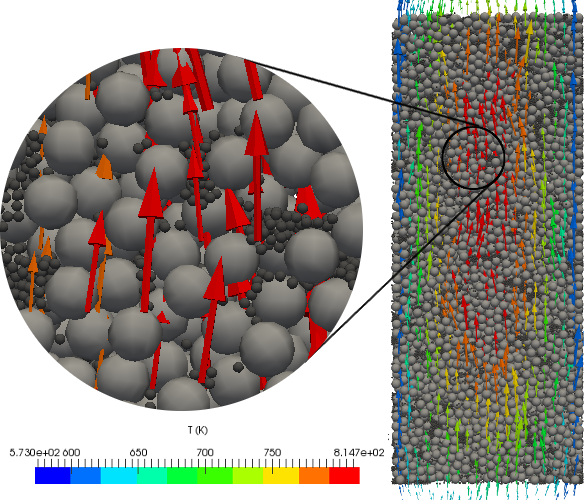
\includegraphics[width = 0.75\textwidth]{figures/pebble_inset_2.png}
    \caption{Showing the case for $\phi_2 = 0.64$, $\eta = 5\%$ with fluid velocity vectors colored by temperature. Inset image reveals size discrepancies between fragments and pebbles and the ensemble interaction with fluid flow.}\label{fig:inset}
\end{figure}

Several cross-sections are created at mid-planes in $z$. Representative results are taken from 64\% packings of $\zeta$- and $\chi$-configurations and compared against their respective $\eta = 5\%$, $r_2^*$ conditions, shown in \Cref{fig:1,fig:3}. The numbered zones of the beds will be discussed shortly.

\begin{figure}[!ht]
    \centering
    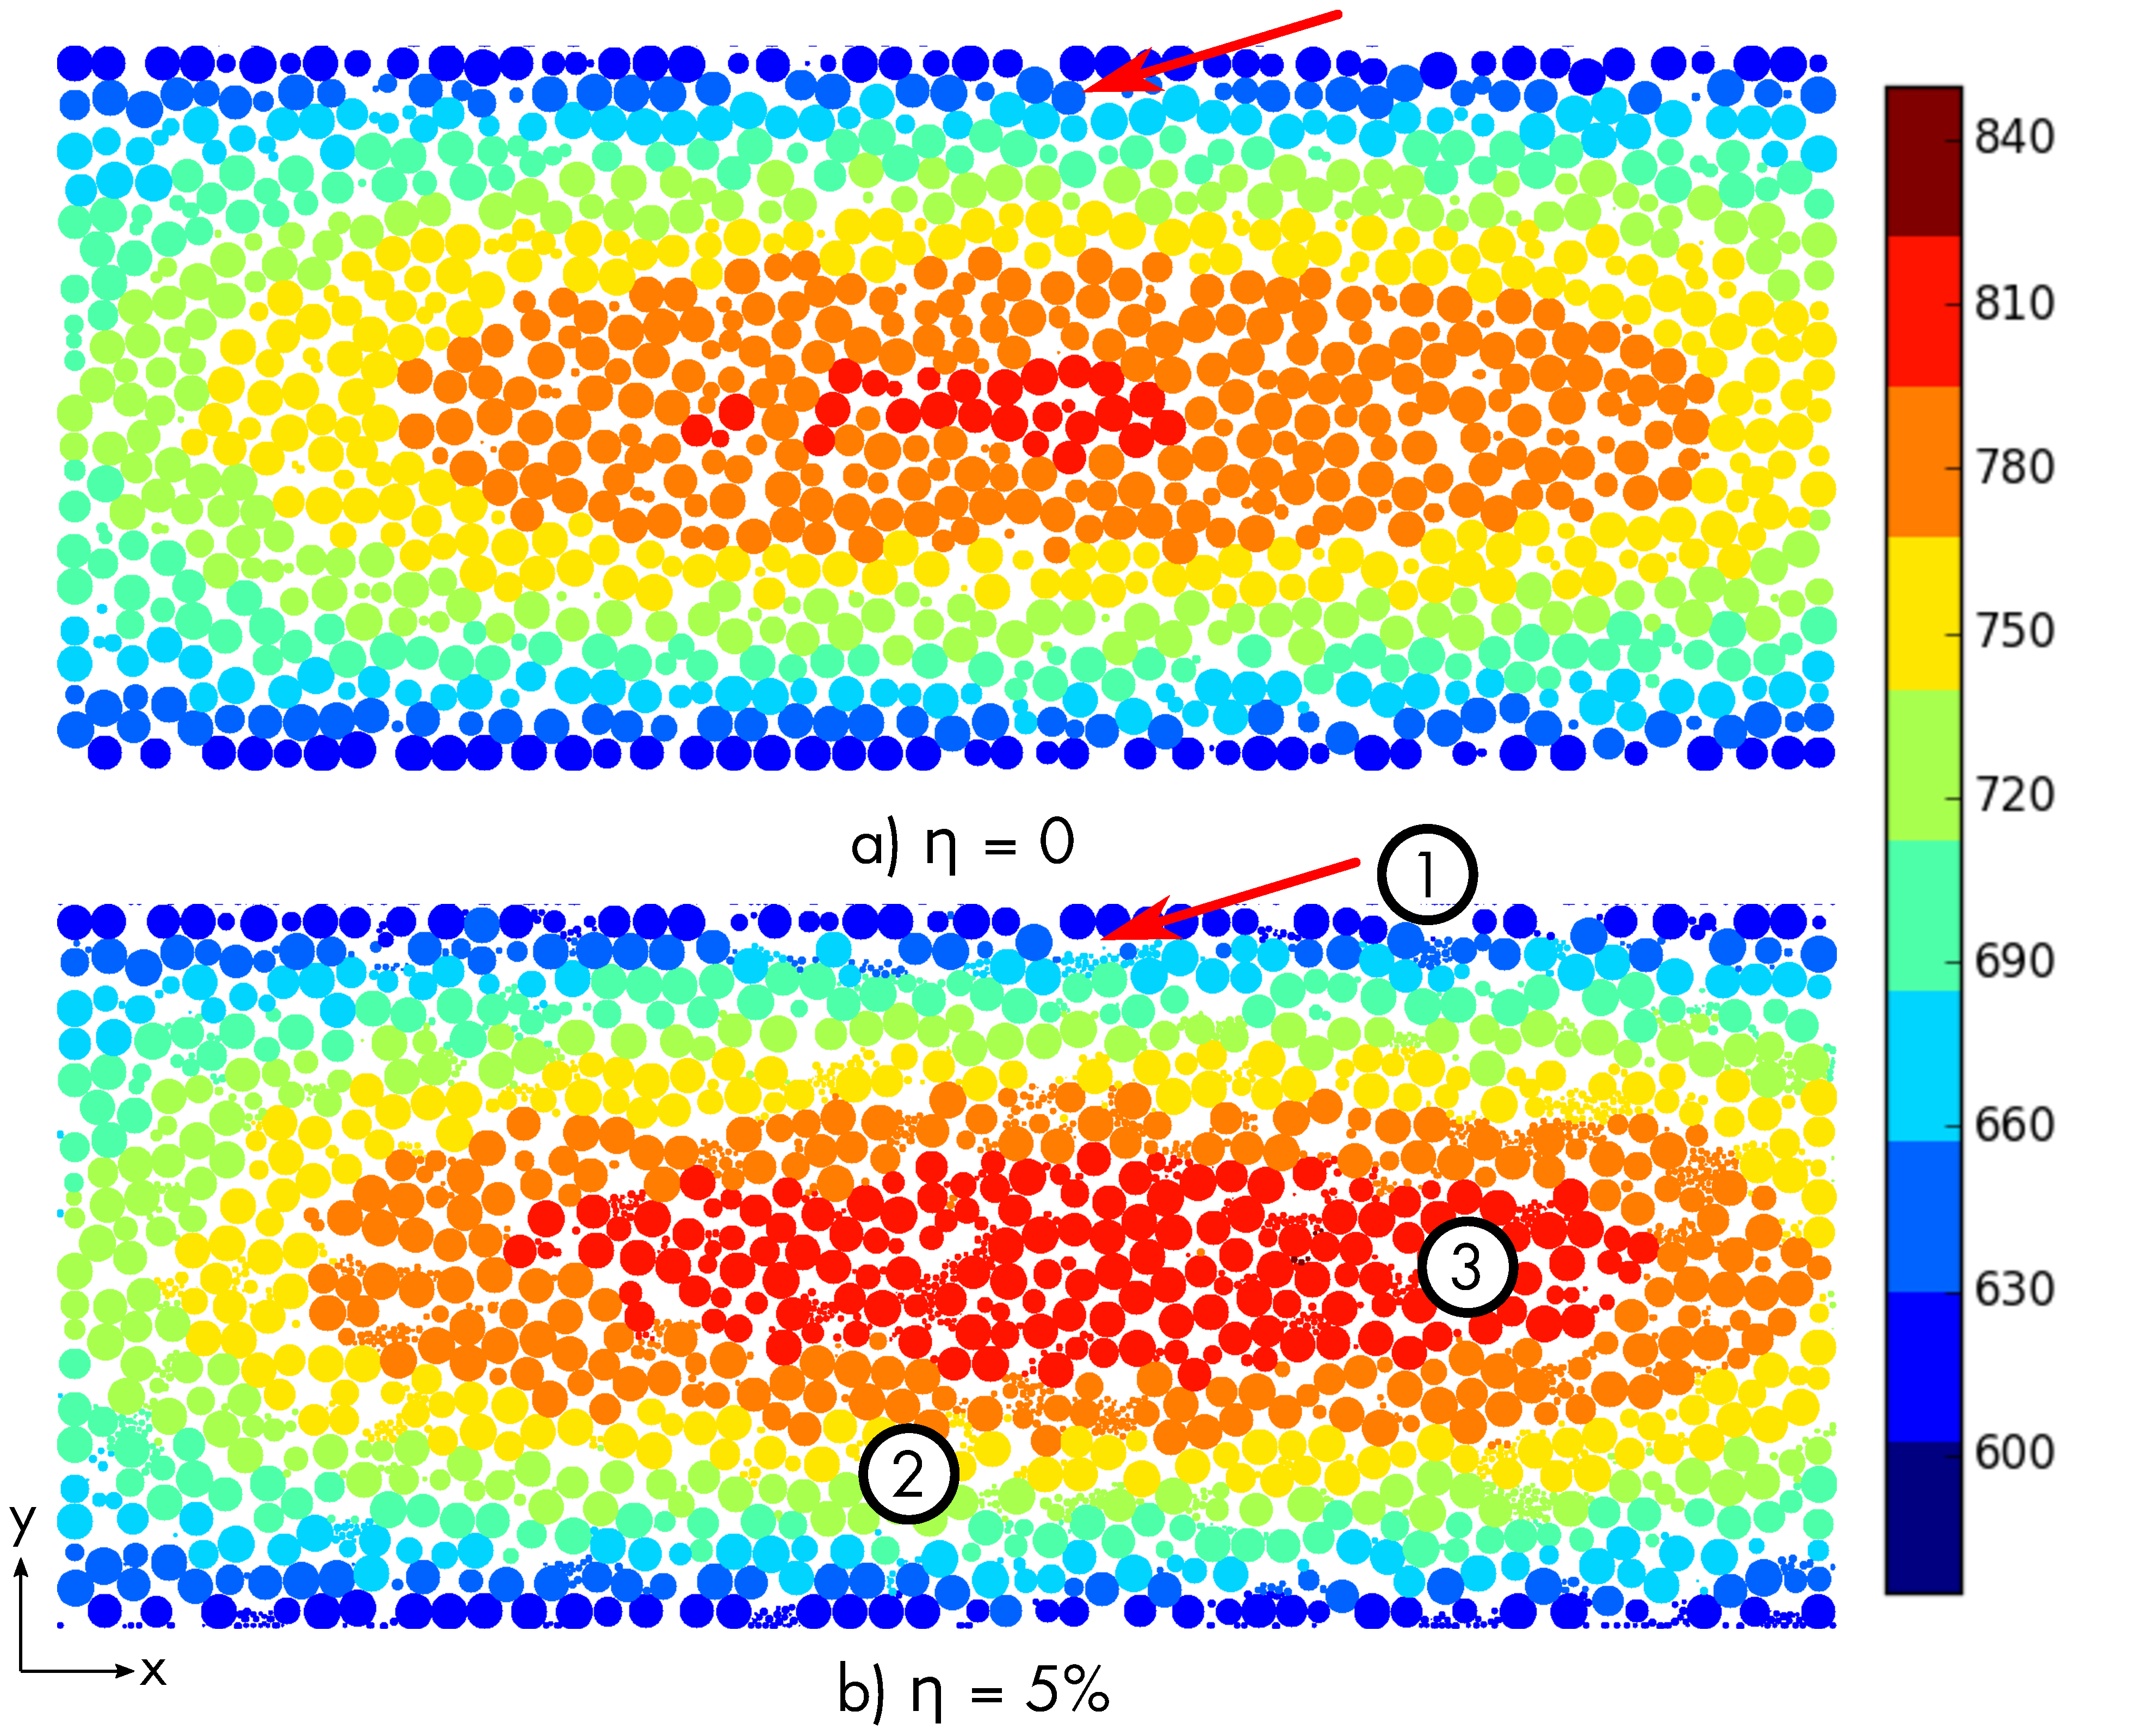
\includegraphics[width = \textwidth]{figures/z-64-discrete.eps}
    \caption{Cuts at the mid-plane of $z$ for $\zeta$-config beds. (a) bed initially packed to $\phi_2$, and (b) bed with crushing of $\eta_5$ pebbles with particle size $r_2^*$. Three important zones have been identified}\label{fig:1}
\end{figure}

\begin{figure}[!ht]
    \centering
    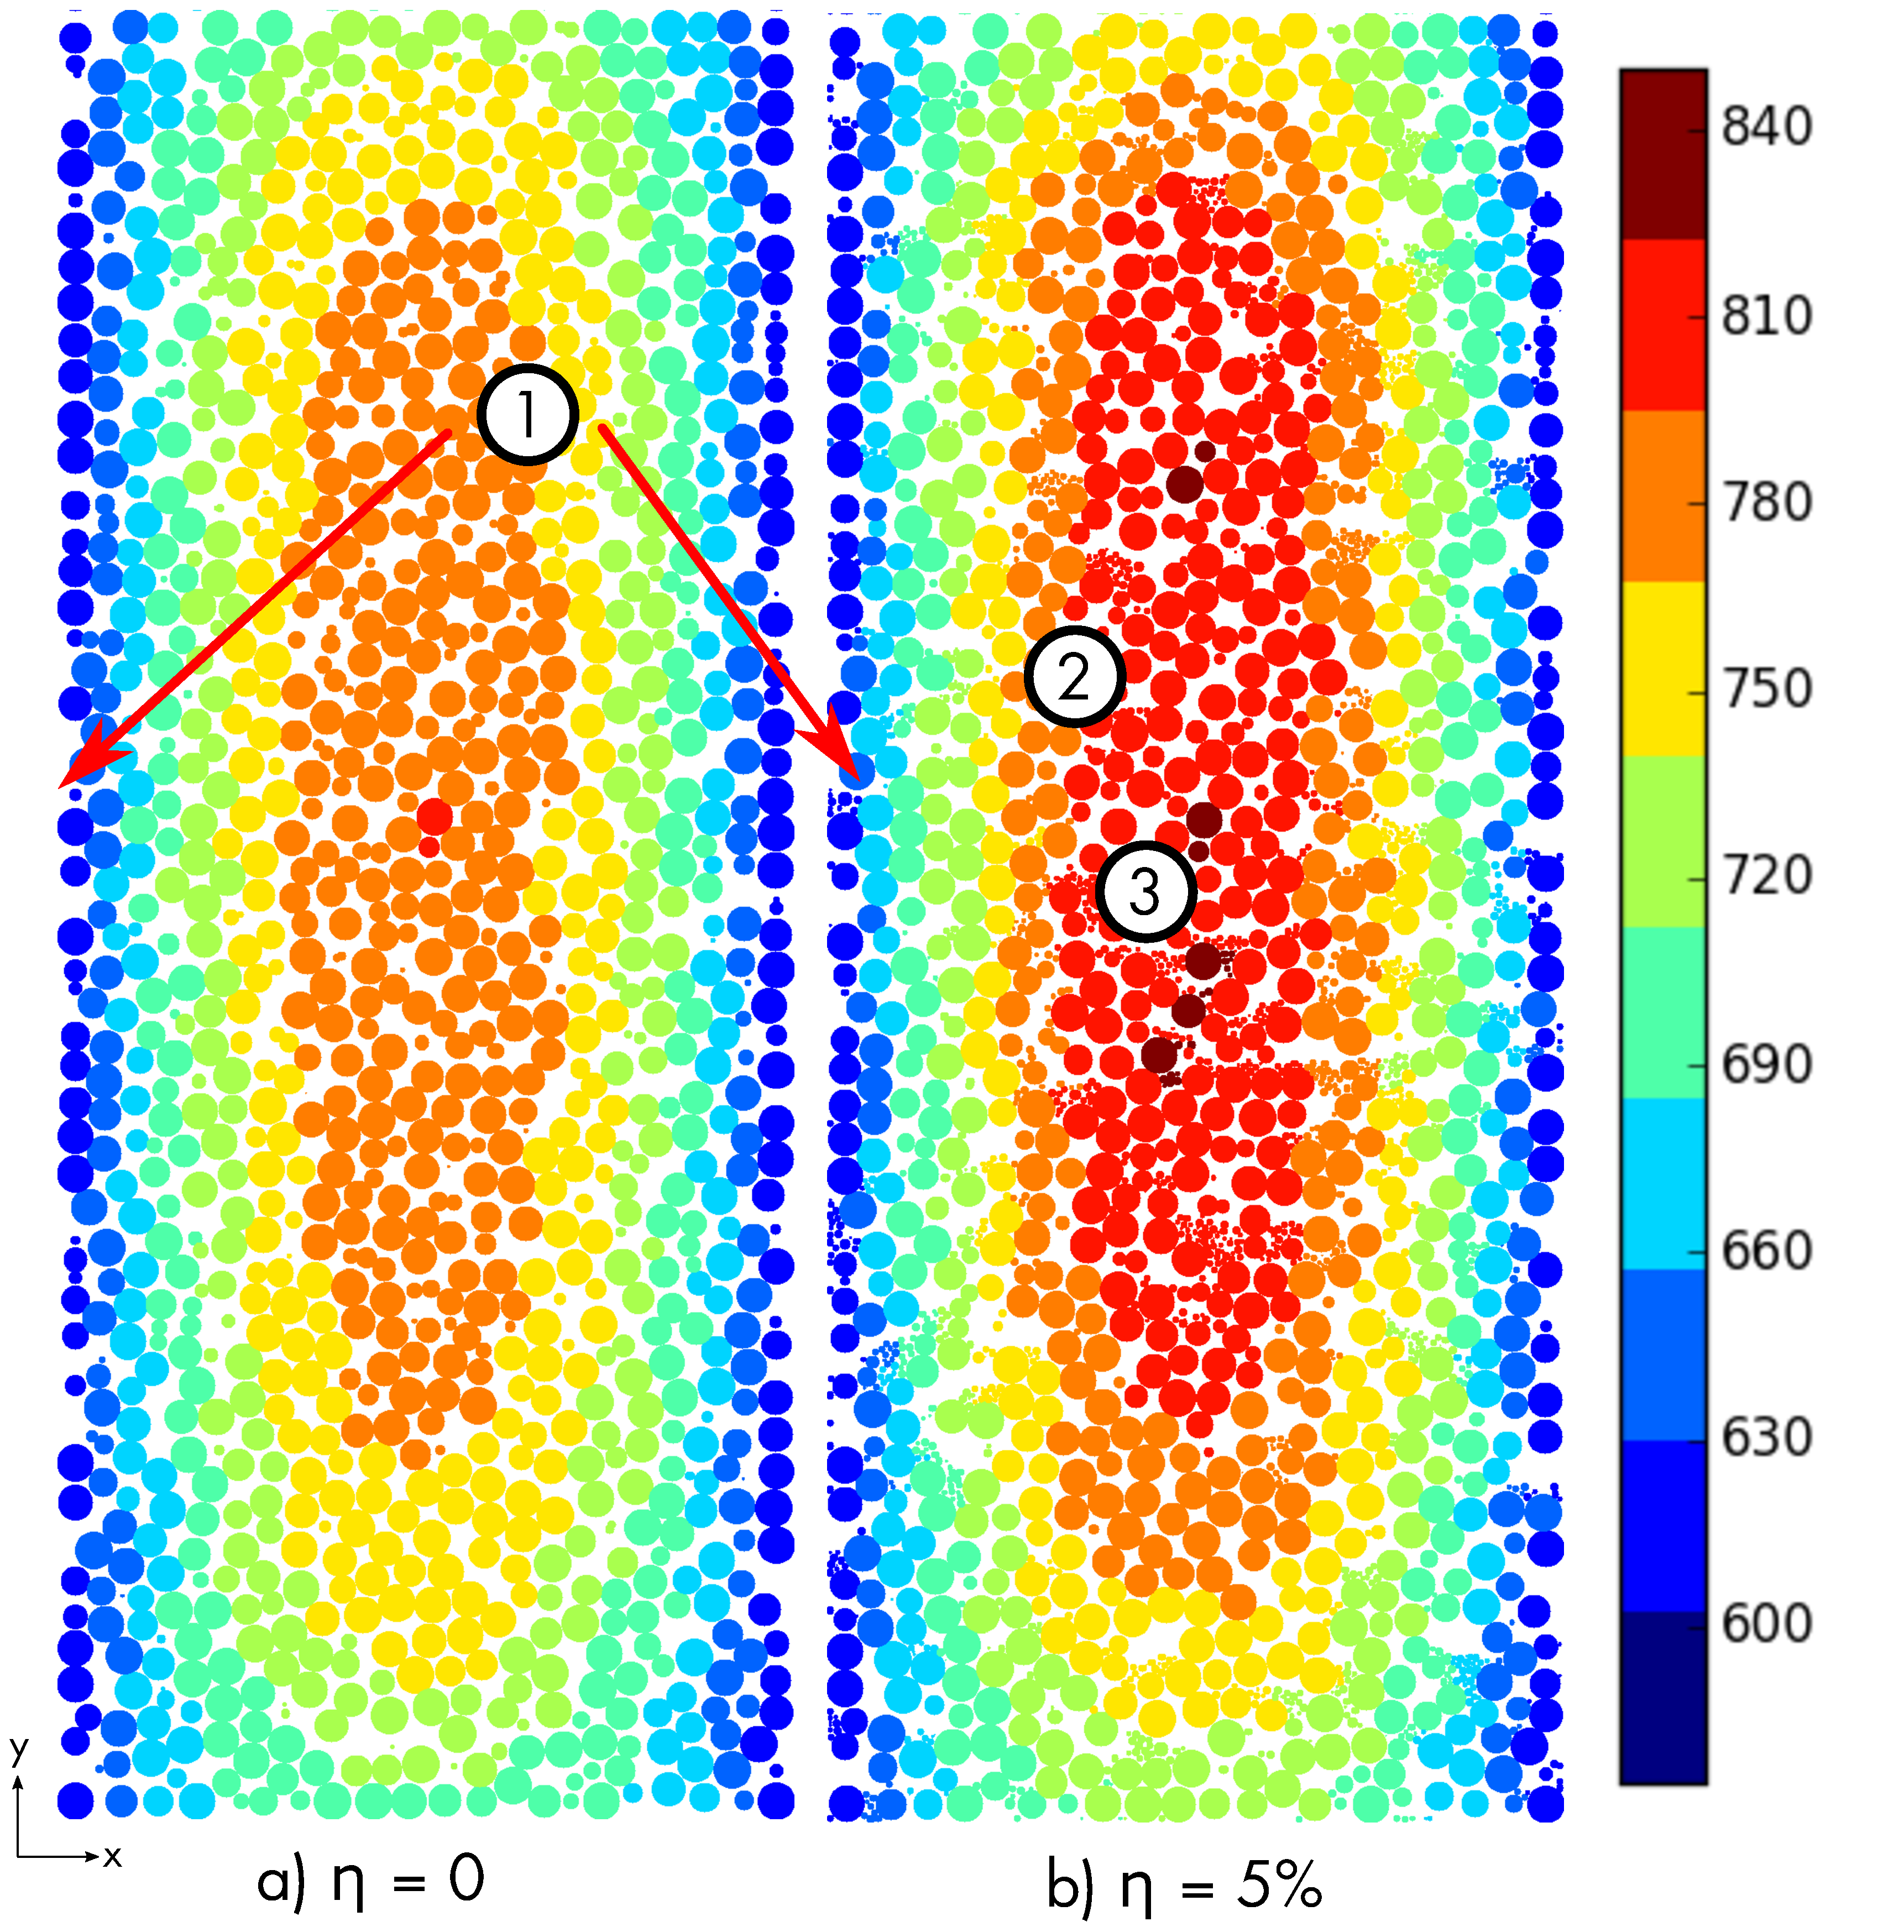
\includegraphics[width = 0.75\textwidth]{figures/x-64-discrete.eps}
    \caption{Cuts at the mid-plane of $z$ for $\chi$-config beds. (a) bed initially packed to $\phi_2$, and (b) bed with crushing of $\eta_5$ pebbles with particle size $r_2^*$. Three important zones have been identified}\label{fig:3}
\end{figure}

Mean reduced temperatures in beds are found in slices of width $\Delta\zeta$ along $\zeta$. Pebble-weighted mean values are found as $\langle T\rangle = \frac{1}{V_n}\sum_{j}^n (T_j-T_w) V_j$, for $n$ pebbles of temperature $T_j$ consuming a total volume $V_n$ in the slice. Demonstrative cases of $\phi_2 = 0.64$ with $r_2^* = 0.2$ are given in \Cref{fig:64-T-profile} as functions of granular crushing percentage.

Pebble bed internal stresses are found from normal and tangential forces that make up force networks in ensembles. Following the formulations described by Gan \& Kamlah \cite{Gan:2010uq}, the magnitude of the stress tensor, $|\sigma|$, is found for every pebble bed at steady-state heating and then normalized against initial ($\eta=0$) beds for respective configurations, given in \Cref{fig:eta-sigma}.%considered configuration, $\sigma^*=|\sigma|_\eta/|\sigma|_{\eta_0}$. %Normalized bed stresses decrease with increasing granular fragmentation, as seen in \Cref{fig:eta-sigma}, for all initial packings and bed orientations, by about 30 to 60\%.

A total mean bed temperature is found from all pebbles in the system as $\langle T\rangle_{tot} = \frac{1}{V_N}\sum_{j}^N (T_j-T_w) V_j$ where $N$ is the total number of ensemble pebbles. The total mean bed temperature is also normalized against initial packing cases of each respective set of beds. Results for all beds are given in \Cref{fig:eta-theta}. Maximum temperature rises of every bed are also found, $T_m = \max(T) - T_w$, and normalized against the maximum temperature in the initial packing of each respective set of beds. To avoid aberrent results from a bed which might have a single, very high temperature pebble, the maximum temperature, $\max(T)$, is calculated as a mean value of the 50 highest temperature pebbles. The results are given in \Cref{fig:eta-T_max}. In addition to total mean bed temperature, maximum temperature rise is also an important factor in evaluation of a pebble bed.

Lastly, we consider how far pebble fragments travel in the bed after a crushing event. Total displacements from the moment of crush event to final resting, $|\Delta h|$, are normalized against the original pebble diameter, $|\Delta h|/d_p$. Histograms for 64\% packing fractions of $\chi$- and $\zeta$-configurations at 5\% pebble crushing are given in \Cref{fig:displacement_hists}. These two beds saw the most settling, all other beds tested saw considerably less fragment displacements.





% \begin{figure}[ht]
% \centering
% 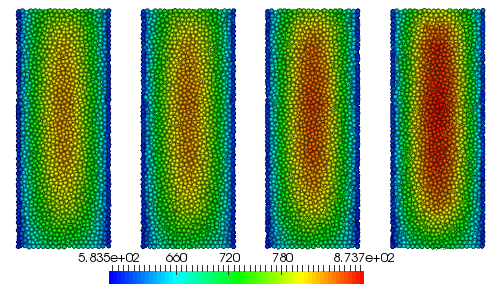
\includegraphics[width = 0.4\textwidth]{figures/62x-edit.png}
% \caption{Pebble temperature distributions in the $\chi$-config with $\phi_1 = 0.62$ initial packing increase with increased granular damage, from left to right is $\eta = 0, 0.01, 0.03, 0.05$.}\label{fig:62xpebs}
% \end{figure}

% numeric integration of mean temperature profiles, $\Theta = \frac{1}{L}\int\langle T \rangle \,\mathrm{d}\zeta$, where $L$ is the \SI{20}{\milli\meter} width of $\zeta$; $\Theta$ is plotted in \Cref{fig:eta-theta}.



% \begin{figure*}[!ht]
%        \centering
%        \begin{subfigure}[b]{0.45\textwidth}
%                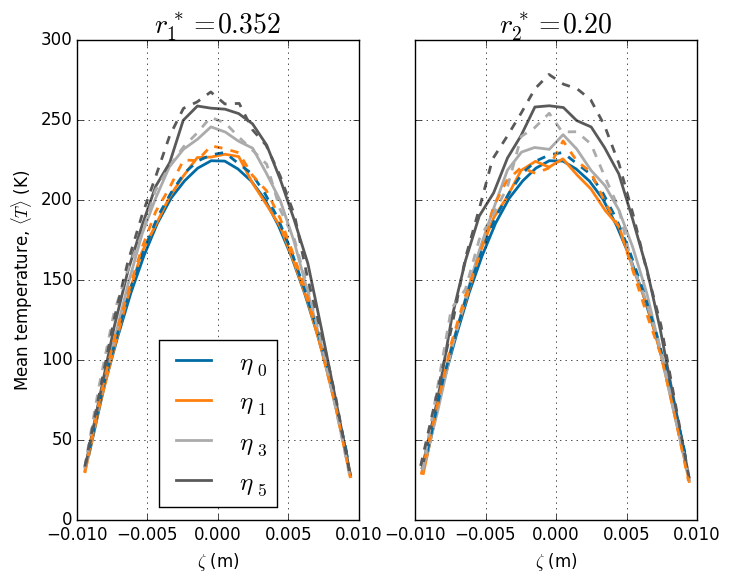
\includegraphics[width=\textwidth]{figures/62-percent-T-profiles.png}
%                \caption{Initial packing fraction of $\phi_1 = 0.62$.}
%                \label{fig:62-T-profile}
%        \end{subfigure}%
%        ~ %add desired spacing between images, e. g. ~, \quad, \qquad, \hfill etc.
%          %(or a blank line to force the subfigure onto a new line)
%        \begin{subfigure}[b]{0.45\textwidth}
%                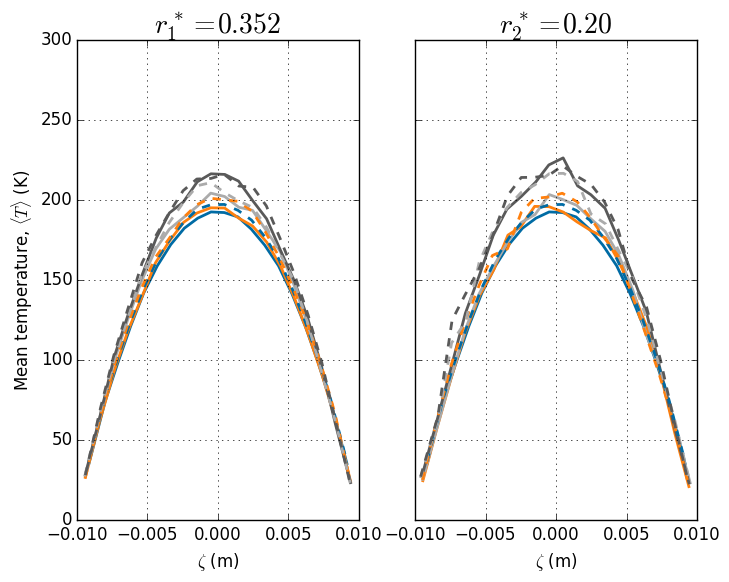
\includegraphics[width=\textwidth]{figures/64-percent-T-profiles.png}
%                \caption{Initial packing fraction of $\phi_2 = 0.64$.}
%                \label{fig:64-T-profile}
%        \end{subfigure}
%        \caption{Solid lines are cases where gravity is in the $\chi$ direction, dashed lines for gravity in the $\zeta$ direction; color is by percent of crushed pebbles, $\eta$.}
% \label{fig:T-profiles}
% \end{figure*}

%

% \begin{figure*}[!ht]
%        \centering
%        \begin{subfigure}[b]{0.45\textwidth}
%                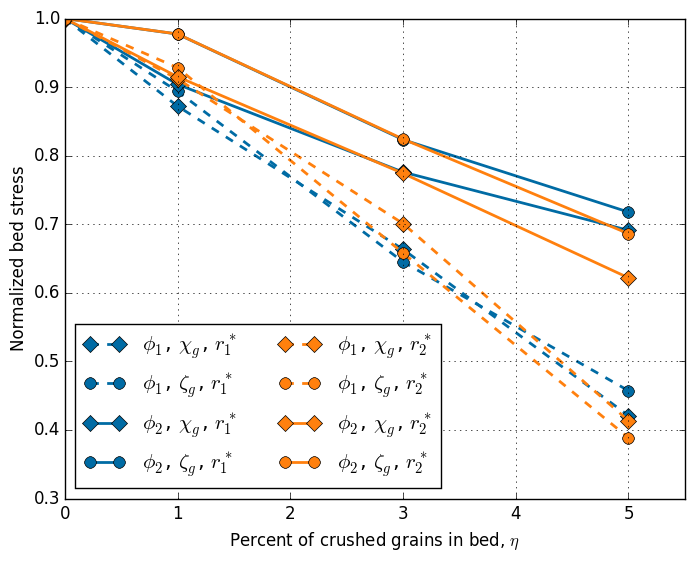
\includegraphics[width = \textwidth]{figures/eta-sigma.png}
%               \caption{Lower packing fractions have lower initial bed stress, stress decreases with increased granular crushing. }\label{fig:eta-sigma}
%        \end{subfigure}%
%        ~ %add desired spacing between images, e. g. ~, \quad, \qquad, \hfill etc.
%          %(or a blank line to force the subfigure onto a new line)
%        \begin{subfigure}[b]{0.45\textwidth}
%                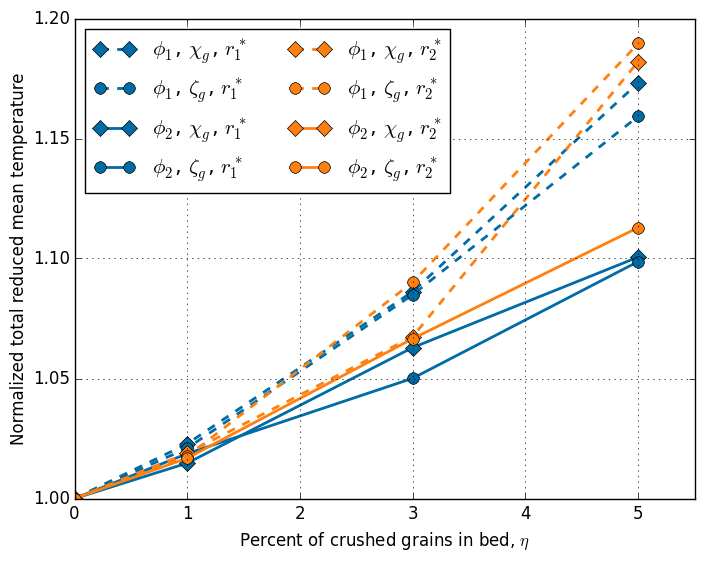
\includegraphics[width = \textwidth]{figures/eta-theta.png}
%               \caption{Lower packing fractions have higher initial bed temperatures, mean temperatures increase with increased granular crushing.}\label{fig:eta-theta}
%        \end{subfigure}
%        \caption{Changes in temperature and bed stress as functions of granular damage percent, $\eta$, with varying parameters of packing fraction, $\phi_1 = 0.62$, $\phi_2 = 0.64$; fragmentation radius ratio, $r_1^* = 0.52$, $r_2^* = 0.2$; and configuration, $\chi_g$ is $\chi$-config, $\zeta_g$ is $\zeta$-config.}
% \label{fig:eta-plots}
% \end{figure*}


\begin{figure}[!t]
    \centering
    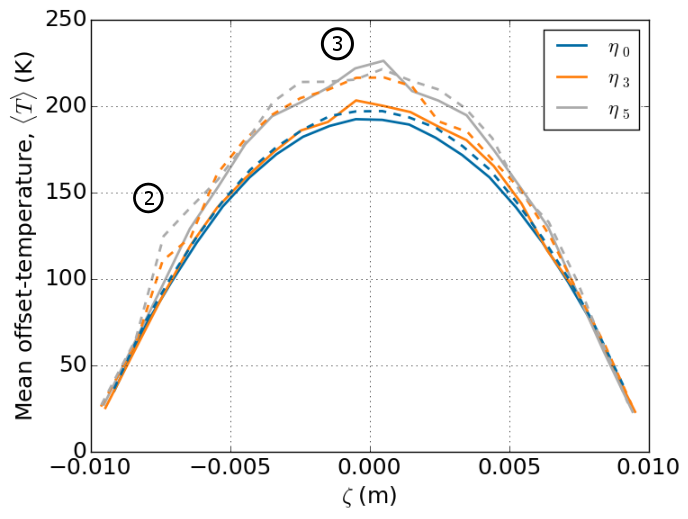
\includegraphics[width=0.5\textwidth]{figures/64-percent-T-profiles-reduced.png}
    \caption{Mean temperature profiles, $\langle T \rangle$, along $\zeta$ in beds with initial packing fractions $\phi_2 = 0.64$, fragmentation sizes were $r_2^*$. Solid lines are $\chi$ configurations, dashes lines are $\zeta$ configurations. Fragmentation settling of $\zeta$-configs are seen in `lumps' near Zone (2) and in the $\chi$-config spike in zone (3).}
    \label{fig:64-T-profile}
\end{figure}

\begin{figure}[!t]
    \centering
    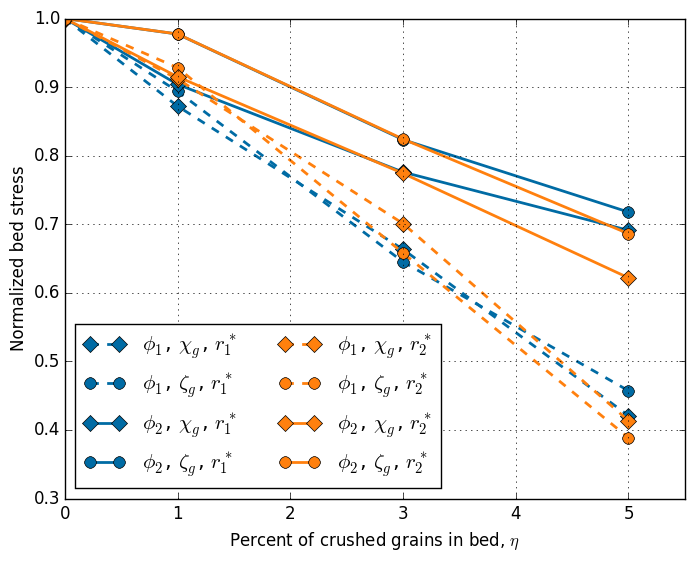
\includegraphics[width = 0.5\textwidth]{figures/eta-sigma.png}
    \caption{Dashed lines represent the lower packing fraction, $\phi_1 = 0.62$, solid lines are $\phi_2 = 0.64$. Markers are: $\circ$ for $\zeta$-config, $\diamondsuit$ for $\chi$-config. Color differentiates the fragment radius ratio. Contact force relaxation is more rapid for lower packing fractions.}\label{fig:eta-sigma}
\end{figure}

\begin{figure}[!t]
    \centering
    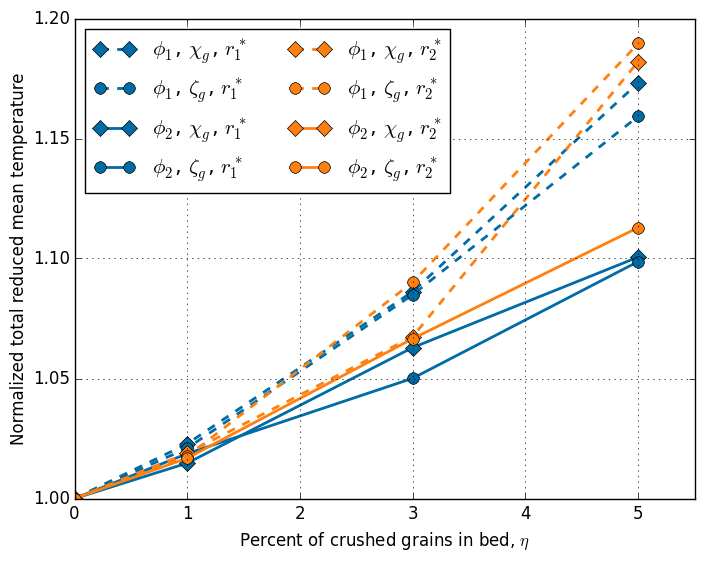
\includegraphics[width = 0.5\textwidth]{figures/eta-theta.png}
    \caption{Dashed lines represent the lower packing fraction, $\phi_1 = 0.62$, solid lines are $\phi_2 = 0.64$. Markers are: $\circ$ for $\zeta$-config, $\diamondsuit$ for $\chi$-config. Color differentiates the fragment radius ratio. Lower packing fraction is the most dominant parameter for overall bed temperature. Amongst the same packing fraction, fragment size is most influential factor.}\label{fig:eta-theta}
\end{figure}

\begin{figure}[!t]
    \centering
    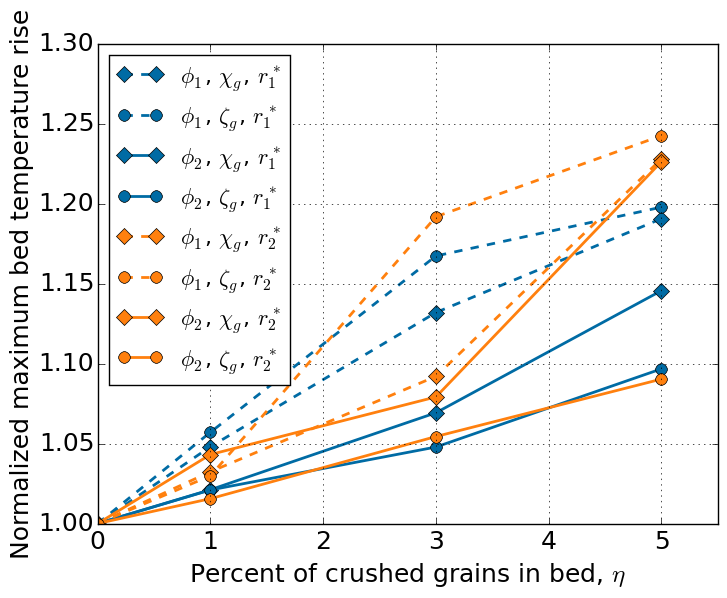
\includegraphics[width = 0.5\textwidth]{figures/eta-T_max.png}
    \caption{Dashed lines represent the lower packing fraction, $\phi_1 = 0.62$, solid lines are $\phi_2 = 0.64$. Markers are: $\circ$ for $\zeta$-config, $\diamondsuit$ for $\chi$-config. Color differentiates the fragment radius ratio. The dominant parameter influencing maximum bed temperature varies as a function of the number of crushed pebbles in the bed.}\label{fig:eta-T_max}
\end{figure}

\begin{figure}[!t]
    \centering
    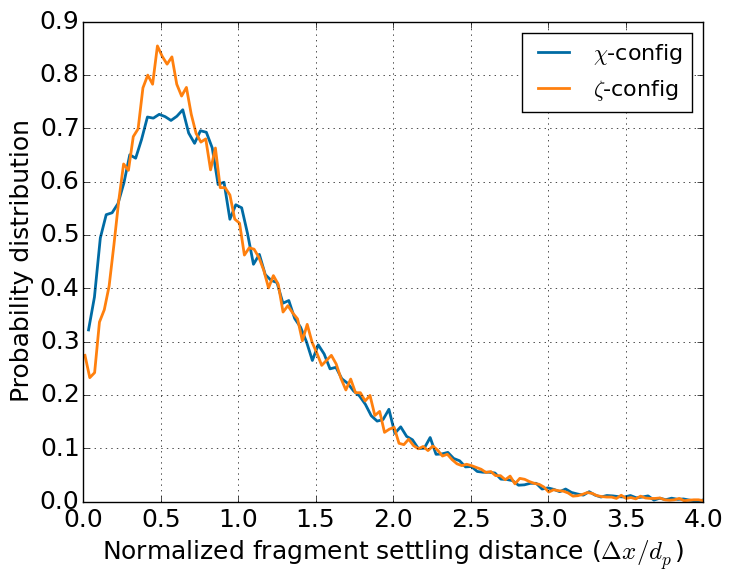
\includegraphics[width = 0.65\textwidth]{figures/displacement_histograms.png}
    \caption{Normalized displacement histograms. $\chi$-config: 59.7\% of fragments travel up to \SI{1}{\milli\meter} and 8.2\% travel more than \SI{2}{\milli\meter}; $\zeta$-config: 60.7\% of fragments travel up to \SI{1}{\milli\meter}, 7.9\% travel more than \SI{2}{\milli\meter}.}\label{fig:displacement_hists}
\end{figure}

% Conductive heat transport in granular materials is dependent on normal forces between pebbles, and normal forces need not be isotropically distributed through beds. To investigate directional dependence, we calculate angular distributions of granular contacts and forces between every pair of interacting pebbles in the ensemble. Contact angle is measured between vectors pointing between contacting pebbles and $\zeta$. In other words, the most direct path for heat out of the system is along contacts at angles of $\theta=0,\pi$; magnitudes of contact forces around those angles dictate the ability of systems to discharge heat to coolant. A mean contact force, $\langle F_n \rangle$, is found inside wedges of $\Delta\theta$ in the same manner described above for ensemble-averaged temperature values. Mean forces for varying fragmentation amount, fragmentation size, initial packing density, and orientation are plotted in \Cref{fig:force-polars}.
% , the stress tensor, $\mathbf{\sigma}$, is
% \begin{equation}
%   \sigma_{jk} = \frac{1}{V}\left(\sum_c d_0 f^{(n)} n_jn_k + \sum_c d_0 f^{(t)} n_jt_k\right)
% \end{equation}
% where $c$ indicates a contact pair of pebbles, $d_0$ is the separation distance between the centroids of the pebbles, $f^{(n)}$ and $f^{(t)}$ are the projected normal and tangential components of the contact force between the pair, and $\mathbf{n}$ and $\mathbf{t}$ are the normal and tangential unit vectors.
% \begin{figure*}[!tp]
%        \centering
%        \begin{subfigure}[b]{0.45\textwidth}
%                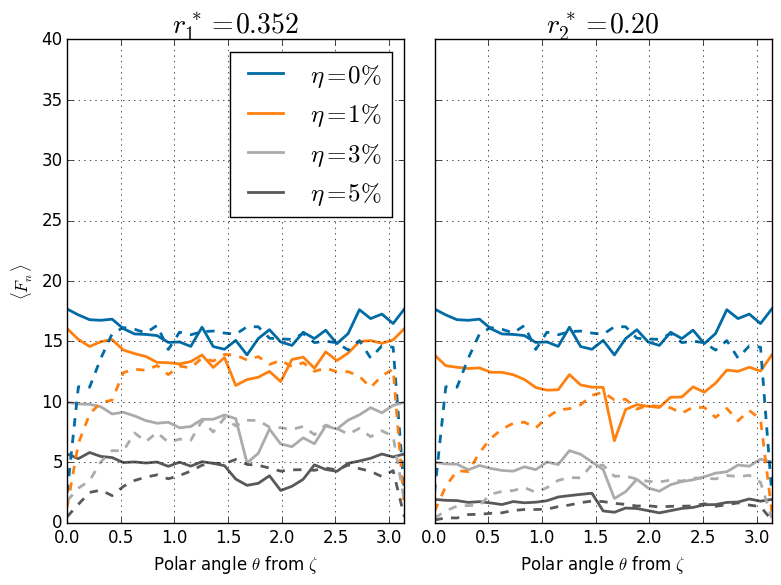
\includegraphics[width=\textwidth]{figures/62-percent-polar-forces.png}
%                \caption{Initial packing fraction of $\phi_1 = 0.62$.}
%                \label{fig:62-force-polar}
%        \end{subfigure}%
%        ~ %add desired spacing between images, e. g. ~, \quad, \qquad, \hfill etc.
%          %(or a blank line to force the subfigure onto a new line)
%        \begin{subfigure}[b]{0.45\textwidth}
%                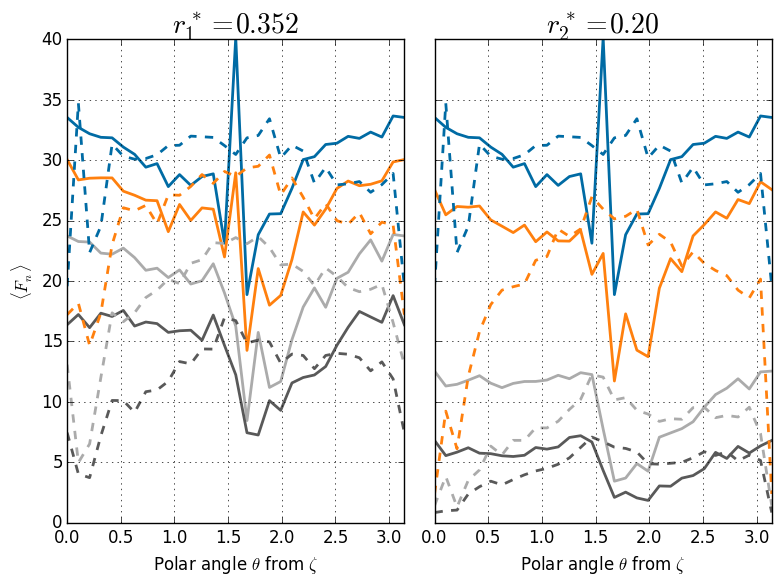
\includegraphics[width=\textwidth]{figures/64-percent-polar-forces.png}
%                \caption{Initial packing fraction of $\phi_2 = 0.64$.}
%                \label{fig:64-force-polar}
%        \end{subfigure}
%        \caption{Ensemble-average contact forces in wedges of angle $\Delta\theta$: solid lines are cases where gravity is in the $\chi$ direction ($\chi$-config), dashed lines for gravity in the $\zeta$ direction ($\zeta$-config); color is by percent of crushed pebbles.} %Grain orientation is such that polar angles of $\theta = 0,\pi$, are the directions of heat transfer in the bed.}
% \label{fig:force-polars}
% \end{figure*}

Analyzing results of all the pebble beds in this study revealed two main contributors to bed temperatures with resettling from pebble crushing: final settling location of fragment particles and overall contact force relaxation. The two interacting contributors were found to be expressed to different extents depending on crush amount and bed configuration.

Bed stress (a global measure of inter-particle contact forces) is predominately a function of initial packing fraction alone, as seen in \Cref{fig:eta-sigma}. Smaller initial packing fractions had their internal stress reduced more rapidly as pebbles crushed in the ensemble. Breeder orientation appears to have less impact on stress relief than size of crush fragments. Due to the inter-connected nature of the force network, and geometry of beds studied here, resettling in beds and contact force relaxation is uniform throughout the beds. Thus we expect reductions in contact forces to directly result in an overall increase of bed temperatures. This is reflected in the curves of \Cref{fig:eta-theta}. Total mean temperatures of $\phi_1 = 0.62$ beds increased between \numrange{16}{19}\% at $\eta = 5\%$. Yet beds initially packed to $\phi_2 = 0.64$ increased by only \numrange{10}{13}\% at the same value of crushed pebble amount.

Fragment settling location, on the contrary, is strongly dependent on fragment size and breeder orientation. The pebble fragments have very poor thermal conductance to neighboring pebbles because they do not exist in the larger pebbles' force network. Fragment temperatures are therefore mostly regulated by convection with interstitial helium and their influence on bed temperatures is much more complex. The effect becomes more pronounced with decreasing size of fragments.

To identify the effects of fragment settling, we look to \Cref{fig:displacement_hists} and the several zones demarcated in the results of \Cref{fig:1,fig:3}. The displacement histogram reveals settling as a relatively localized event. Most fragments, even in this case of smallest fragment size and largest crushing amount, remain approximately at the location of the parent pebble; for both configurations, approximately 60\% travel less than 1 pebble diameter (\SI{1}{\milli\meter}). However, in both configurations, approximately 8\% of fragments travel more than 2 diameters, and those pebbles have a significant impact on the ensembles overall thermal response.

In $\zeta$-configuration beds, pebbles traveling more than a few pebble diameters will move between colored isotherms drawn in \Cref{fig:1}. For example we can see the fragment group identified in Zone (1) as moving downward, away from the top wall. Similarly, when pebbles in Zone (3) are crushed, some of the fragments tumble downward into Zone (2) before coming to rest where they continue to receive volumetric heating. Thus the fragments, with poor thermal conductance, increase heating in the regions where they settle. The effect is seen in the $\eta = 3, 5\%$ temperature profiles in \Cref{fig:64-T-profile} that are asymmetric with lower temperatures in the top half (above Zone (3)) and higher temperatures in the region near Zone (2).

In contrast, $\chi$-config beds respond much differently to pebble fragment settling. We again see from cross-sections in \Cref{fig:3} a pebble identified in Zone (1) that breaks but remains in that zone after settling. The trend continues in other regions of the bed. Because of the gravity's effect, when pebbles are crushed in the $\chi$-config beds, they fall downward but remain generally in the same isotherm, as drawn in \Cref{fig:3}. According to \Cref{fig:64-T-profile}, the effect of pebble crushing has little effect up to 3\% of damaged pebbles. But suddenly at $\eta = 5\%$, the combination of reduced overall bed stress and fragmentation heating causes the maximum bed temperature to jump above all other $\phi = 64\%$ beds (see \Cref{fig:64-T-profile} and \Cref{fig:eta-T_max}). The temperature increase in this $\chi$-config bed is due to the accumulation of pebble fragments that remain in Zone (3), only tumbling to lower heights. Helium that enters the $\chi$-configuration bed reaches higher temperatures more quickly due to the increased heating from fragments which settled at lower heights of $y$. Helium then continues to heat from the many fragments in Zone (3) which ultimately results in the highest maximum bed temperatures (for the given packing fraction). This can also be seen with comparison between \Cref{fig:1,fig:3}: the $\chi$-config bed reaches the $780$~\si{\kelvin} contour at a much lower height than the $\zeta$-configuration. 




\subsubsection{Local Packing Fraction Redistribution}
Travel of pebble fragments also manifests in changes to local packing fraction. In \Cref{fig:x-62-r23,fig:x-62-r125,fig:x-624-r23,fig:x-624r125}, we see the local packing fraction distribution for all pebble beds of $\chi$-configuration. 
\begin{figure}[!t]
    \centering
    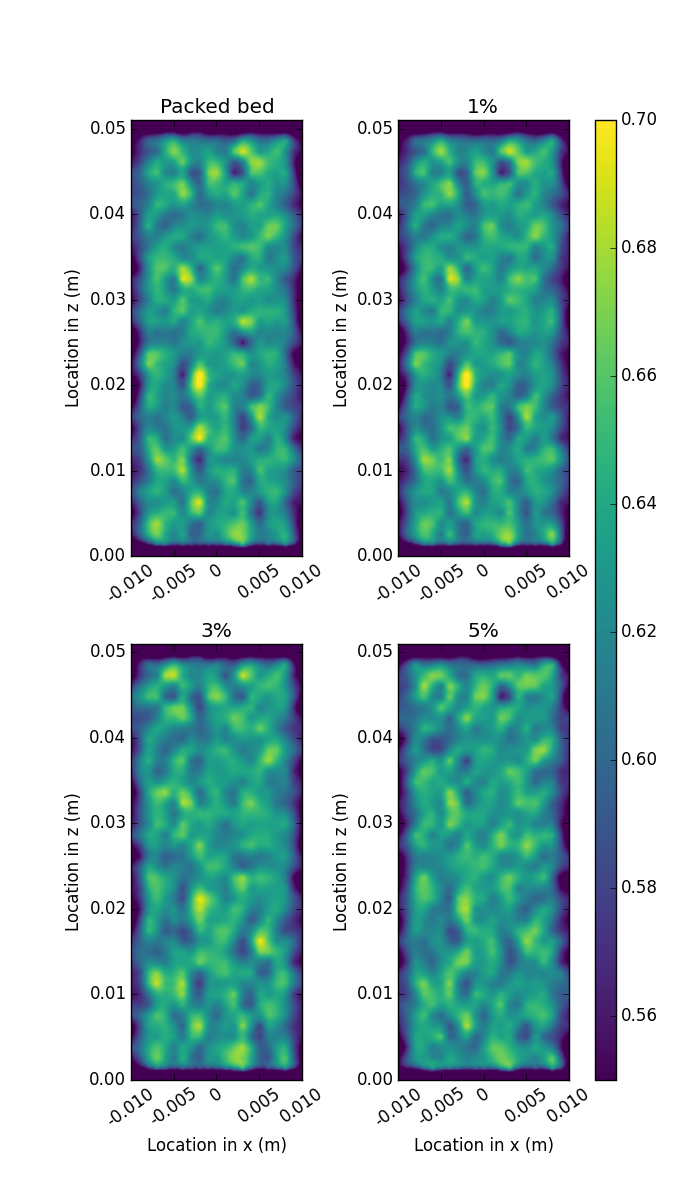
\includegraphics[width = 0.65\textwidth]{figures/x-62-r23-1.png}
    \caption{Distribution of local packing fraction for $\chi$-config, $\phi = 0.62$, $r^* = 0.32$}\label{fig:x-62-r23}
\end{figure}

\begin{figure}[!t]
    \centering
    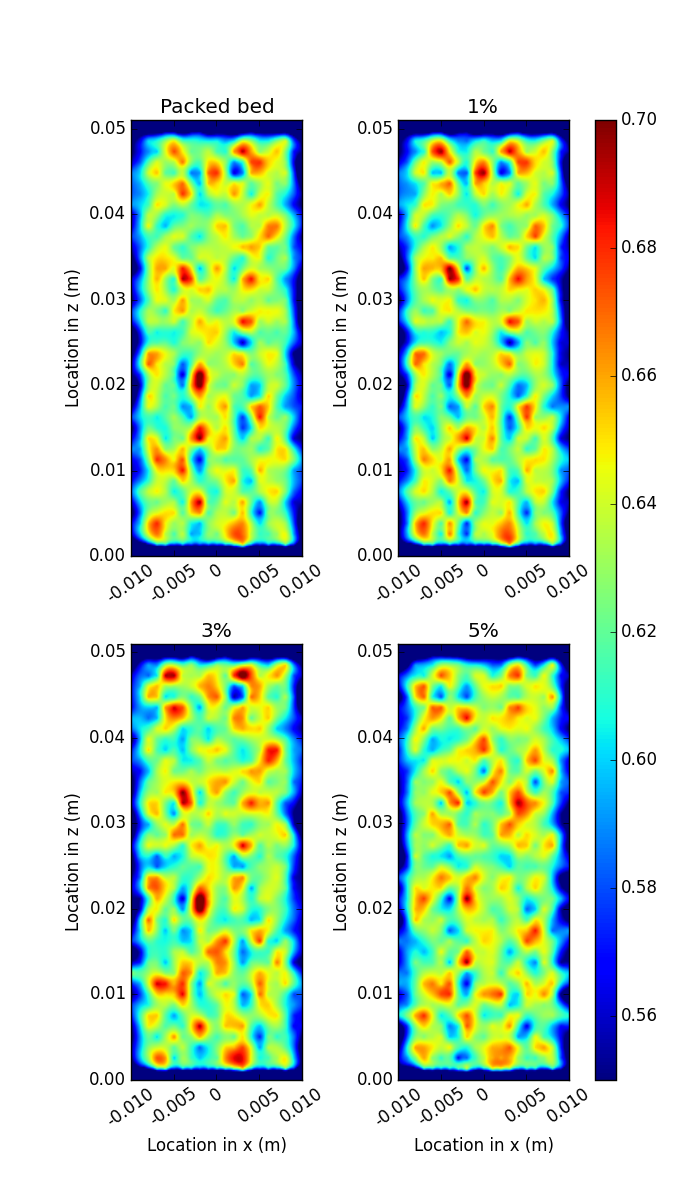
\includegraphics[width = 0.65\textwidth]{figures/x-62-r125-1.png}
    \caption{Distribution of local packing fraction for $\chi$-config, $\phi = 0.62$, $r^* = 0.2$}\label{fig:x-62-r125}
\end{figure}

\begin{figure}[!t]
    \centering
    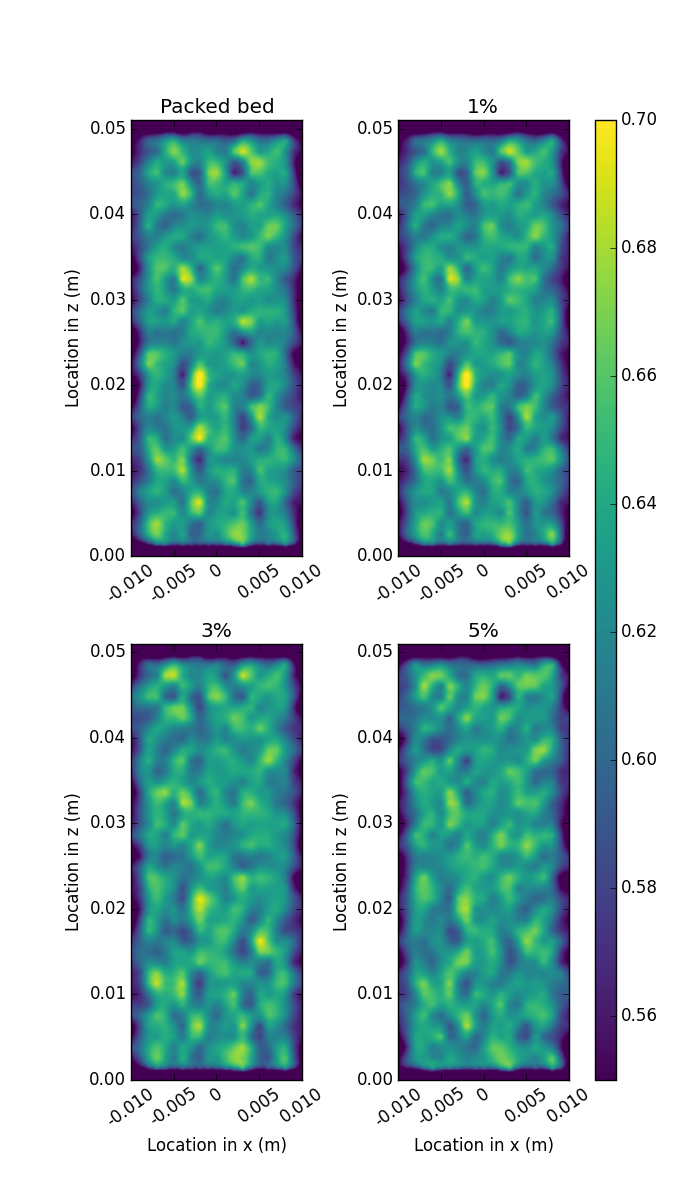
\includegraphics[width = 0.65\textwidth]{figures/x-62-r23-1.png}
    \caption{Distribution of local packing fraction for $\chi$-config, $\phi = 0.64$, $r^* = 0.32$}\label{fig:x-624-r23}
\end{figure}
\begin{figure}[!t]
    \centering
    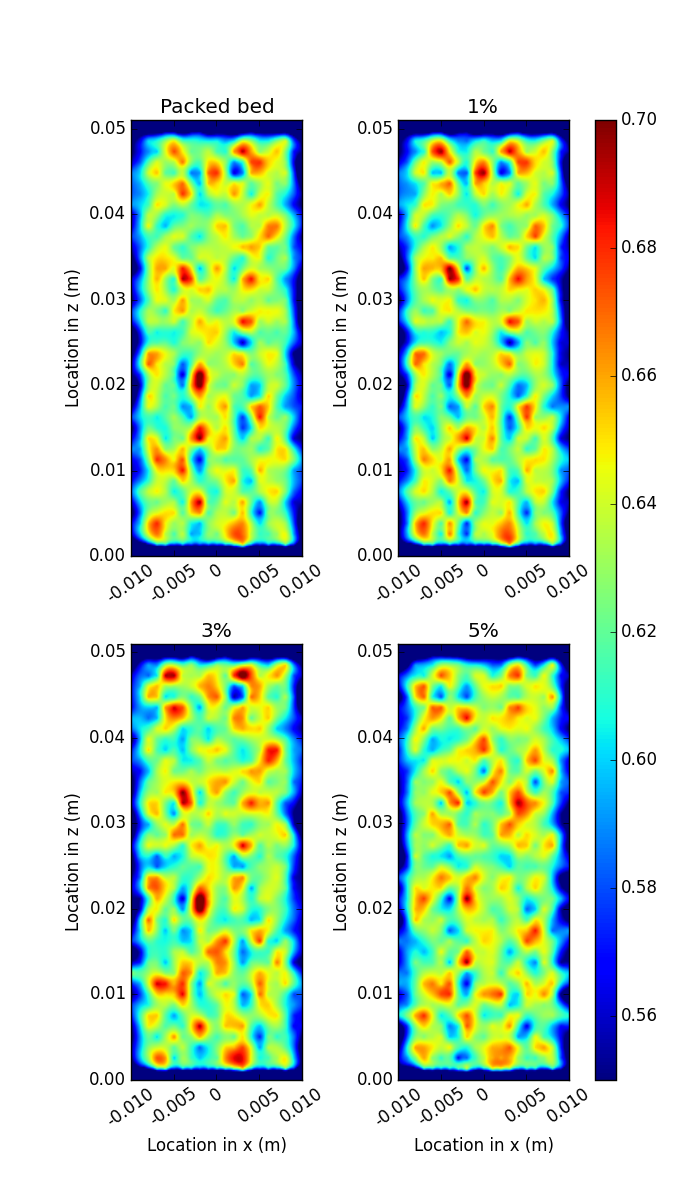
\includegraphics[width = 0.65\textwidth]{figures/x-62-r125-1.png}
    \caption{Distribution of local packing fraction for $\chi$-config, $\phi = 0.64$, $r^* = 0.2$}\label{fig:x-624r125}
\end{figure}


% deltas~~~~~~~~~~~~~~~~~~~~~~~~~~
\begin{figure}[!t]
    \centering
    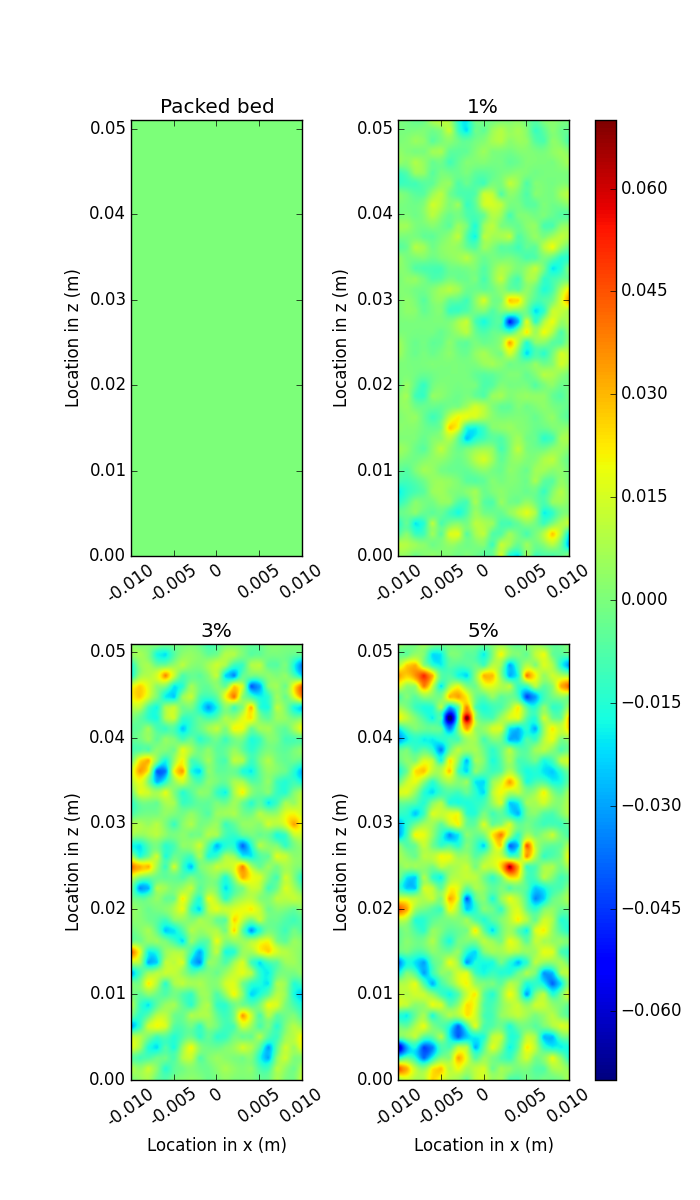
\includegraphics[width = 0.65\textwidth]{figures/x-62-r23-1-deltas.png}
    \caption{Distribution of local changes in packing fraction ($\phi_eta - \phi_i$) for $\chi$-config, $\phi = 0.62$, $r^* = 0.32$}\label{fig:x-62-r23-deltas}
\end{figure}

\begin{figure}[!t]
    \centering
    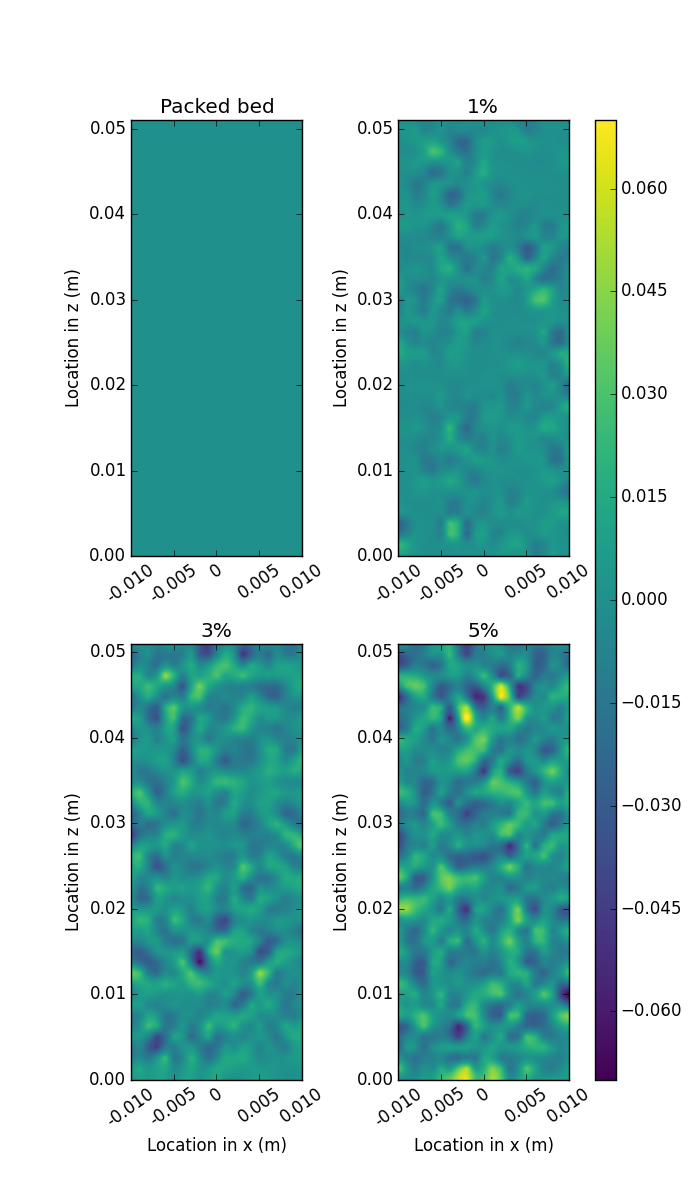
\includegraphics[width = 0.65\textwidth]{figures/x-62-r125-1-deltas.png}
    \caption{Distribution of local changes in packing fraction ($\phi_eta - \phi_i$) for $\chi$-config, $\phi = 0.62$, $r^* = 0.2$}\label{fig:x-62-r125-deltas}
\end{figure}

\begin{figure}[!t]
    \centering
    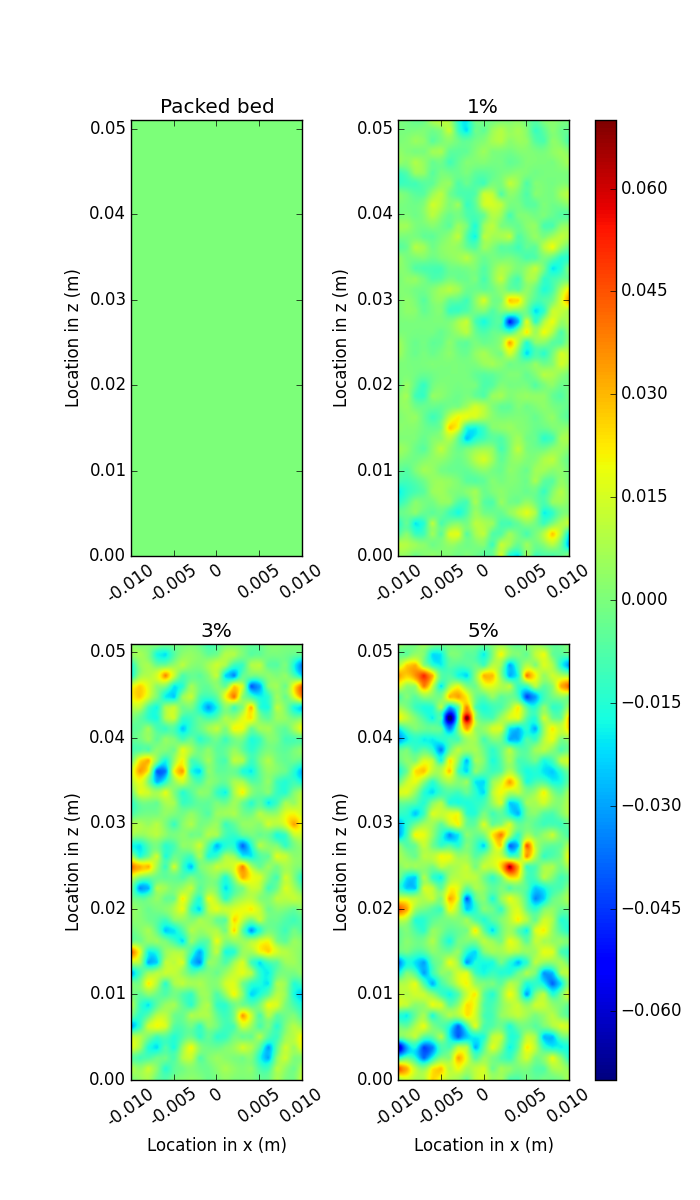
\includegraphics[width = 0.65\textwidth]{figures/x-62-r23-1-deltas.png}
    \caption{Distribution of local changes in packing fraction ($\phi_eta - \phi_i$) for $\chi$-config, $\phi = 0.64$, $r^* = 0.32$}\label{fig:x-624-r23-deltas}
\end{figure}

\begin{figure}[!t]
    \centering
    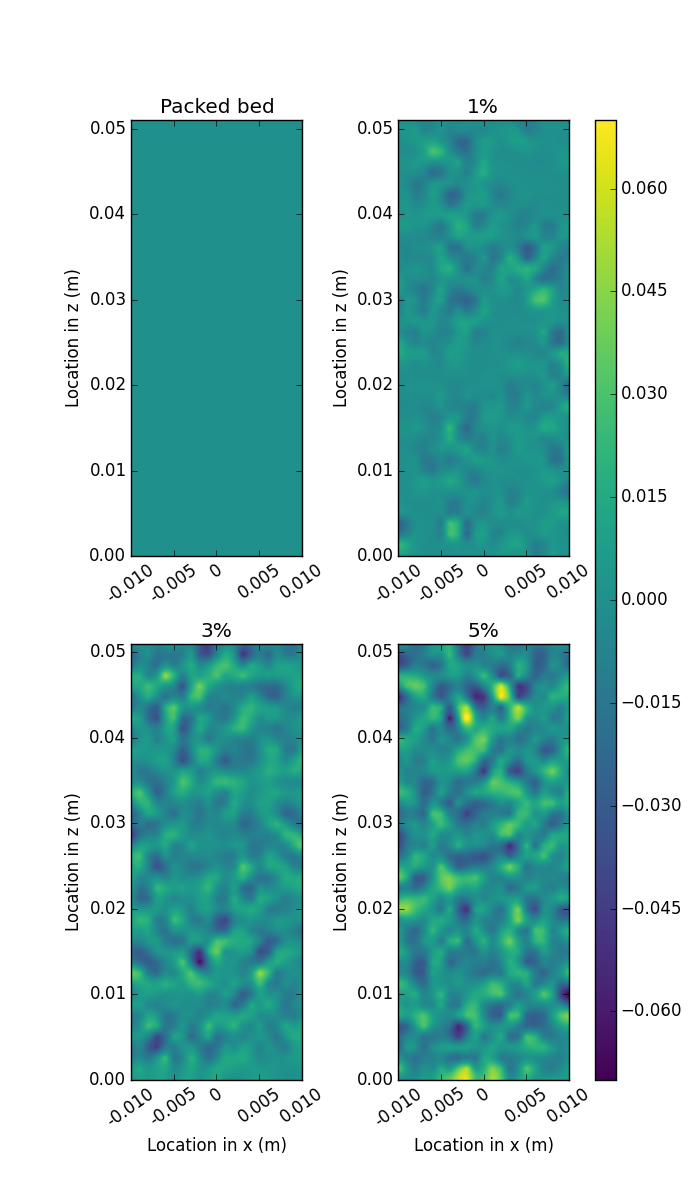
\includegraphics[width = 0.65\textwidth]{figures/x-62-r125-1-deltas.png}
    \caption{Distribution of local changes in packing fraction ($\phi_eta - \phi_i$) for $\chi$-config, $\phi = 0.64$, $r^* = 0.2$}\label{fig:x-624-r125-deltas}
\end{figure}
% deltas~~~~~~~~~~~~~~~~~~~~~~~~~~



\begin{figure}[!t]
    \centering
    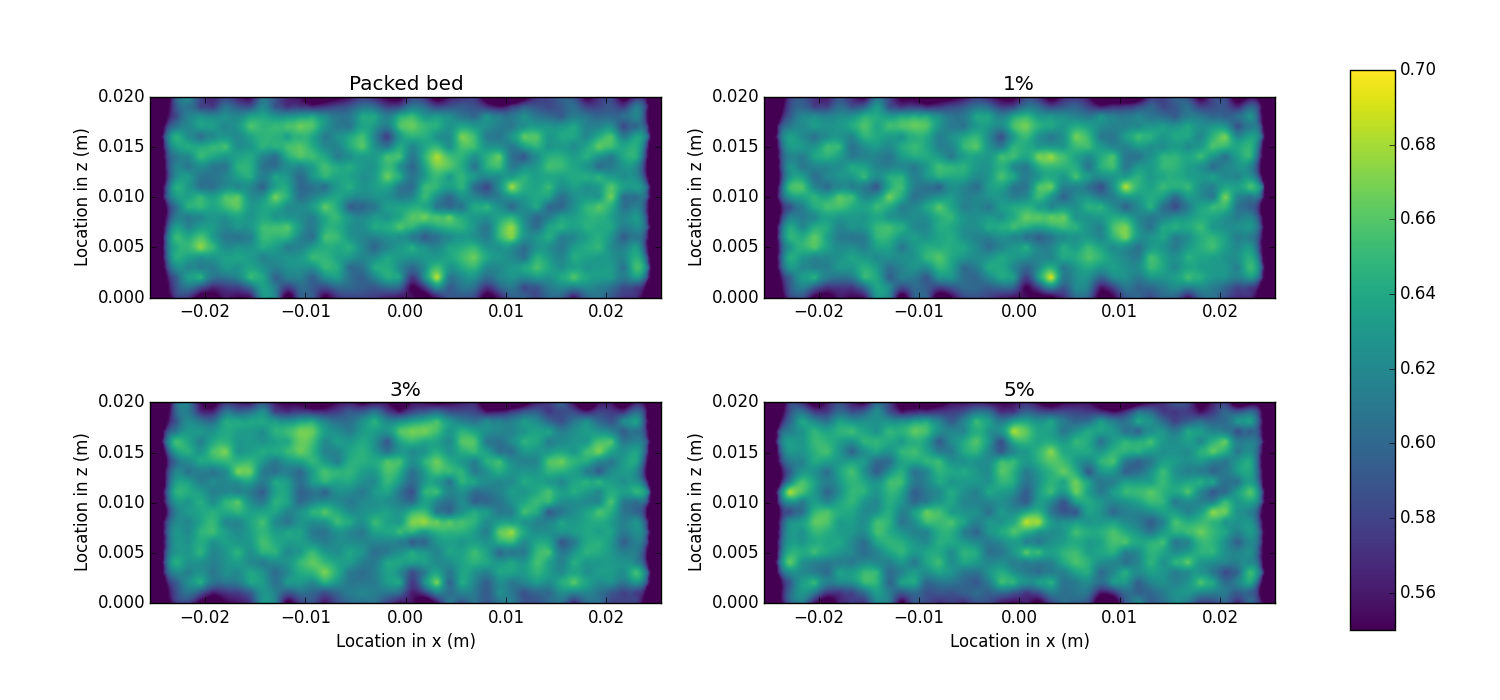
\includegraphics[width = 0.95\textwidth]{figures/z-62-r23-1.png}
    \caption{Distribution of local packing fraction for $\zeta$-config, $\phi = 0.62$, $r^* = 0.32$}\label{fig:z-62-r23}
\end{figure}
\begin{figure}[!t]
    \centering
    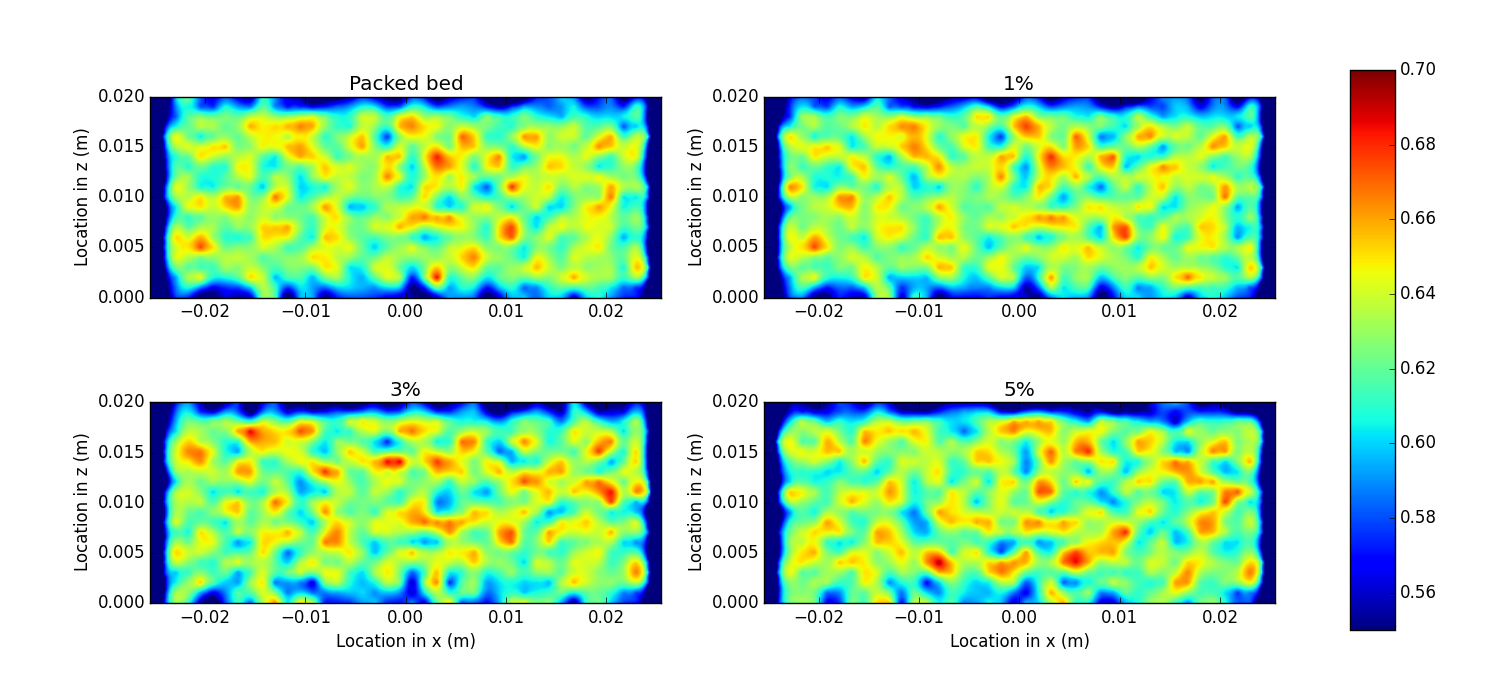
\includegraphics[width = 0.95\textwidth]{figures/z-62-r125-1.png}
    \caption{Distribution of local packing fraction for $\zeta$-config, $\phi = 0.62$, $r^* = 0.2$}\label{fig:z-62-r125}
\end{figure}
\begin{figure}[!t]
    \centering
    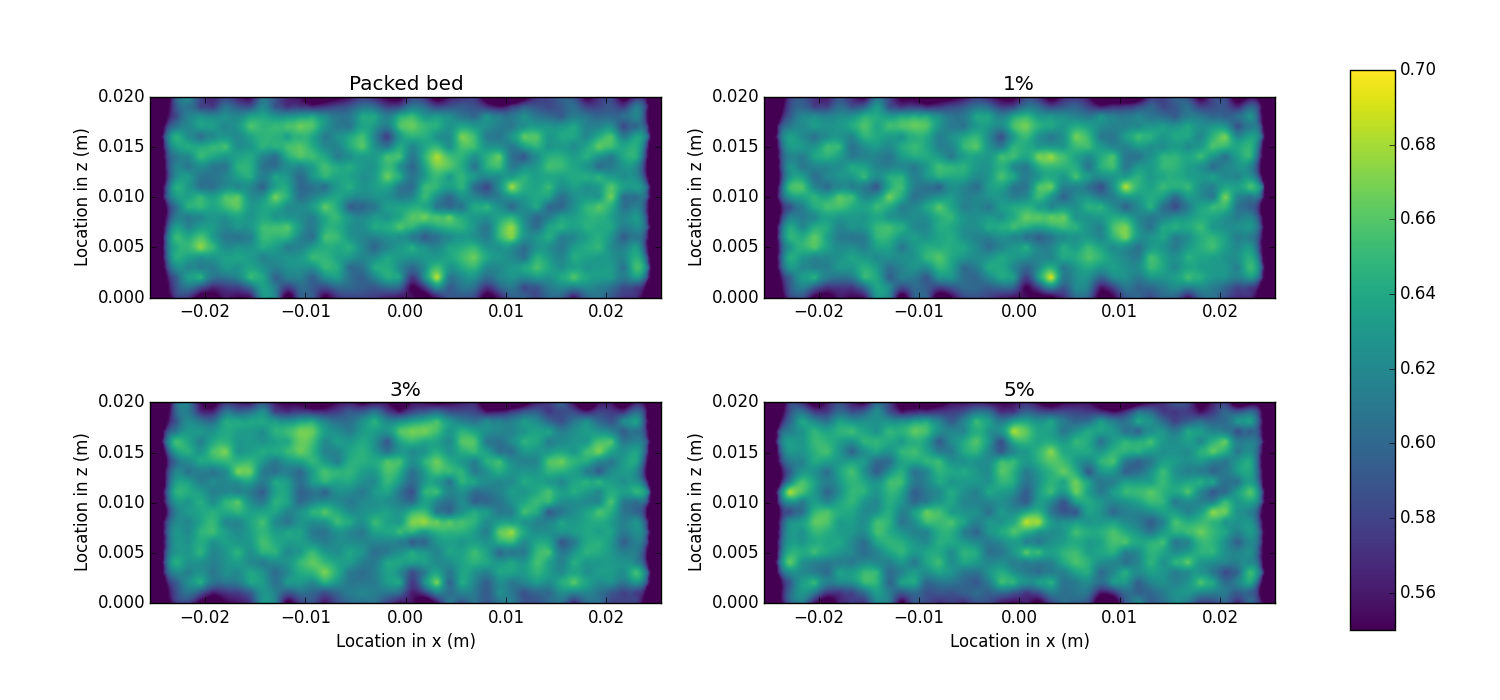
\includegraphics[width = 0.95\textwidth]{figures/z-62-r23-1.png}
    \caption{Distribution of local packing fraction for $\zeta$-config, $\phi = 0.64$, $r^* = 0.32$}\label{fig:z-624-r23}
\end{figure}
\begin{figure}[!t]
    \centering
    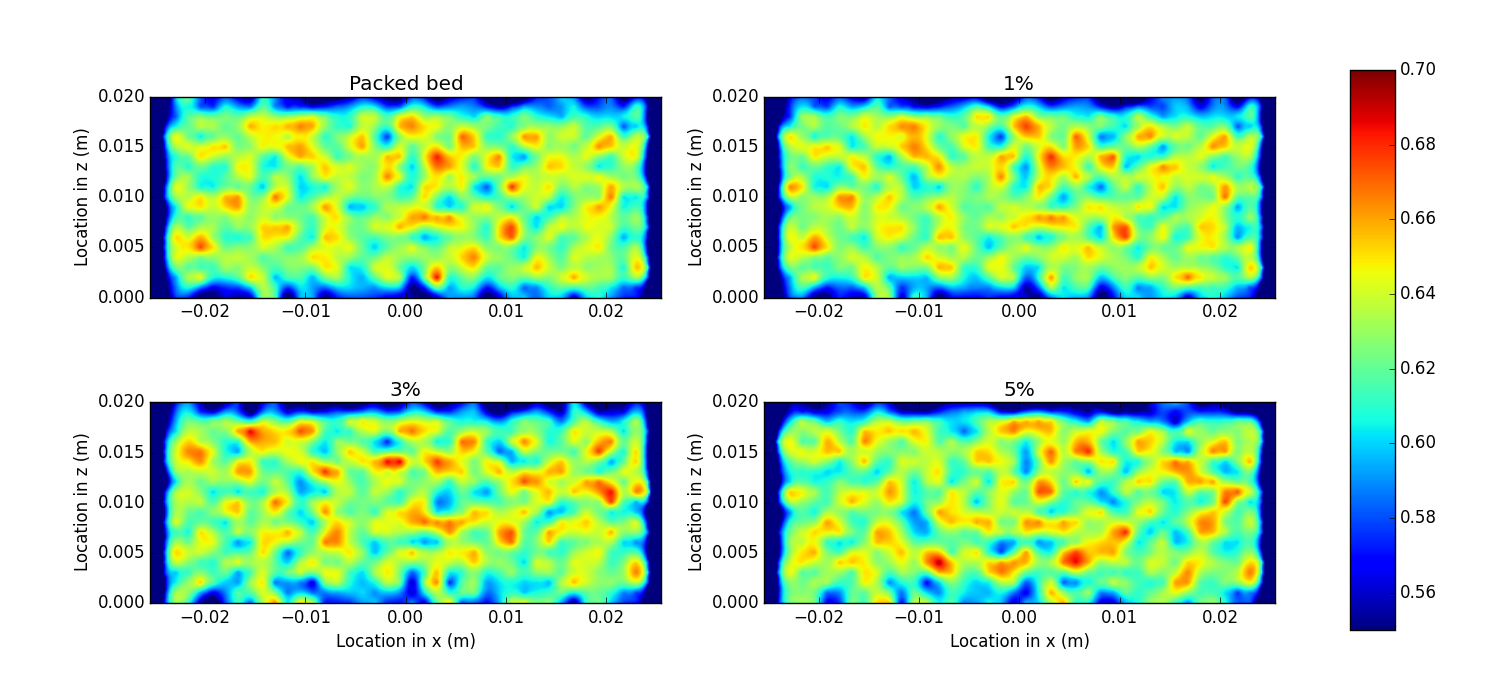
\includegraphics[width = 0.95\textwidth]{figures/z-62-r125-1.png}
    \caption{Distribution of local packing fraction for $\zeta$-config, $\phi = 0.64$, $r^* = 0.2$}\label{fig:z-624r125}
\end{figure}



% deltas~~~~~~~~~~~~~~~~~~~~~~~~~~
\begin{figure}[!t]
    \centering
    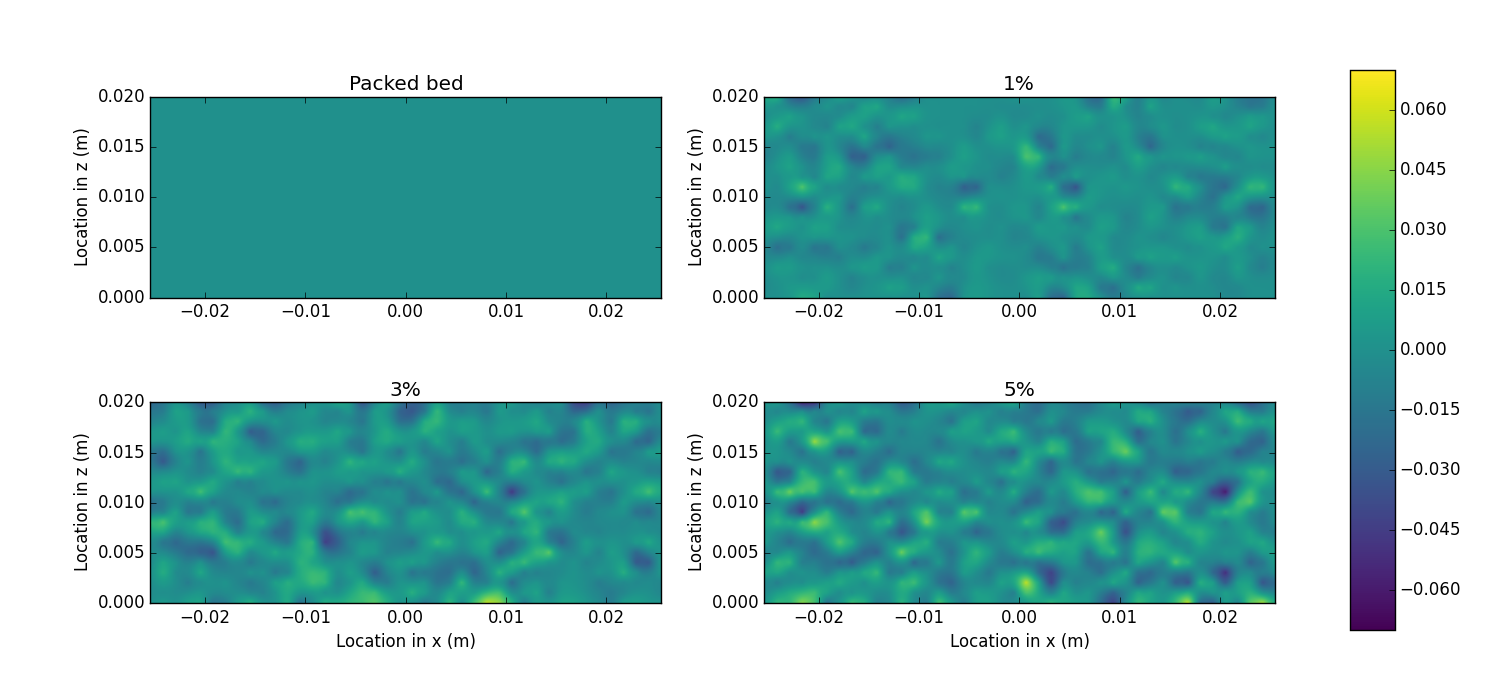
\includegraphics[width = 0.95\textwidth]{figures/z-62-r23-1-deltas.png}
    \caption{Distribution of local changes in packing fraction ($\phi_eta - \phi_i$) for $\zeta$-config, $\phi = 0.62$, $r^* = 0.32$}\label{fig:z-62-r23-deltas}
\end{figure}

\begin{figure}[!t]
    \centering
    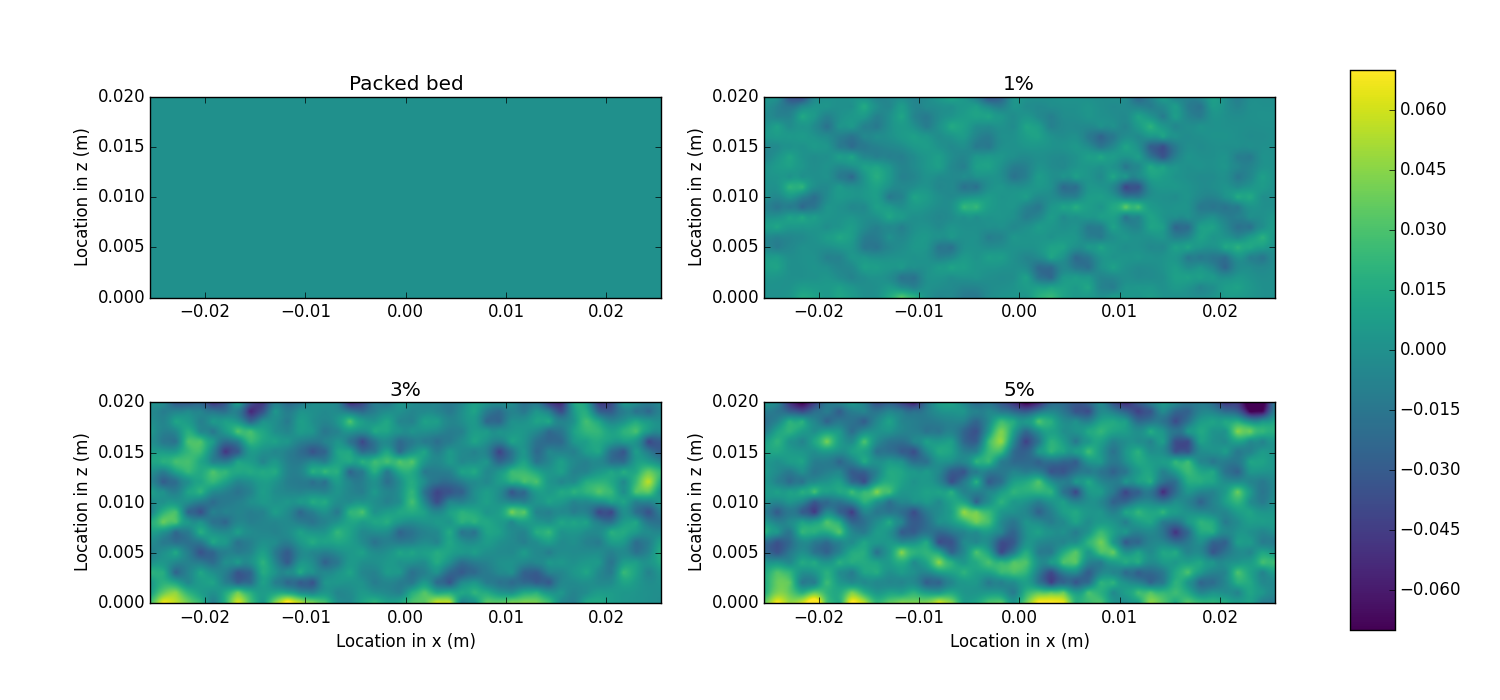
\includegraphics[width = 0.95\textwidth]{figures/z-62-r125-1-deltas.png}
    \caption{Distribution of local changes in packing fraction ($\phi_eta - \phi_i$) for $\zeta$-config, $\phi = 0.62$, $r^* = 0.2$}\label{fig:z-62-r125-deltas}
\end{figure}

\begin{figure}[!t]
    \centering
    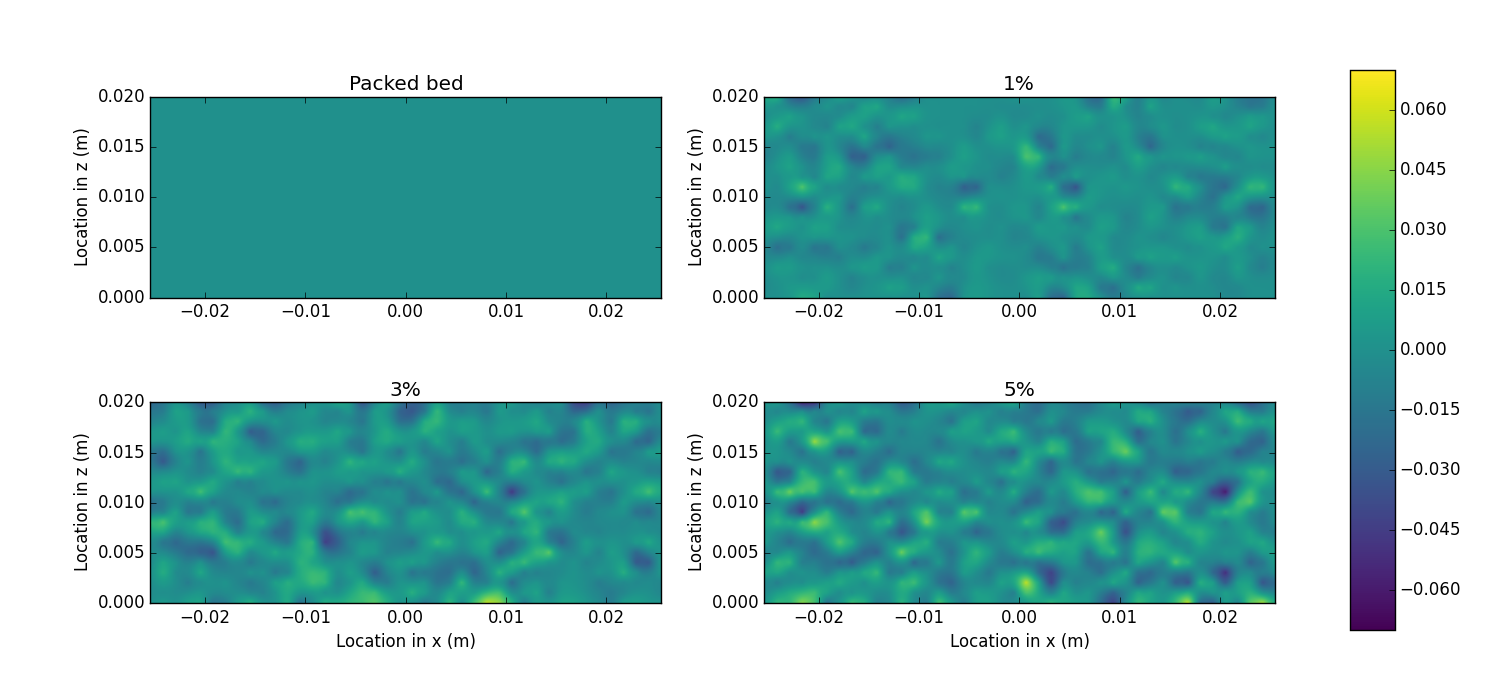
\includegraphics[width = 0.95\textwidth]{figures/z-62-r23-1-deltas.png}
    \caption{Distribution of local changes in packing fraction ($\phi_eta - \phi_i$) for $\zeta$-config, $\phi = 0.64$, $r^* = 0.32$}\label{fig:z-624-r23-deltas}
\end{figure}

\begin{figure}[!t]
    \centering
    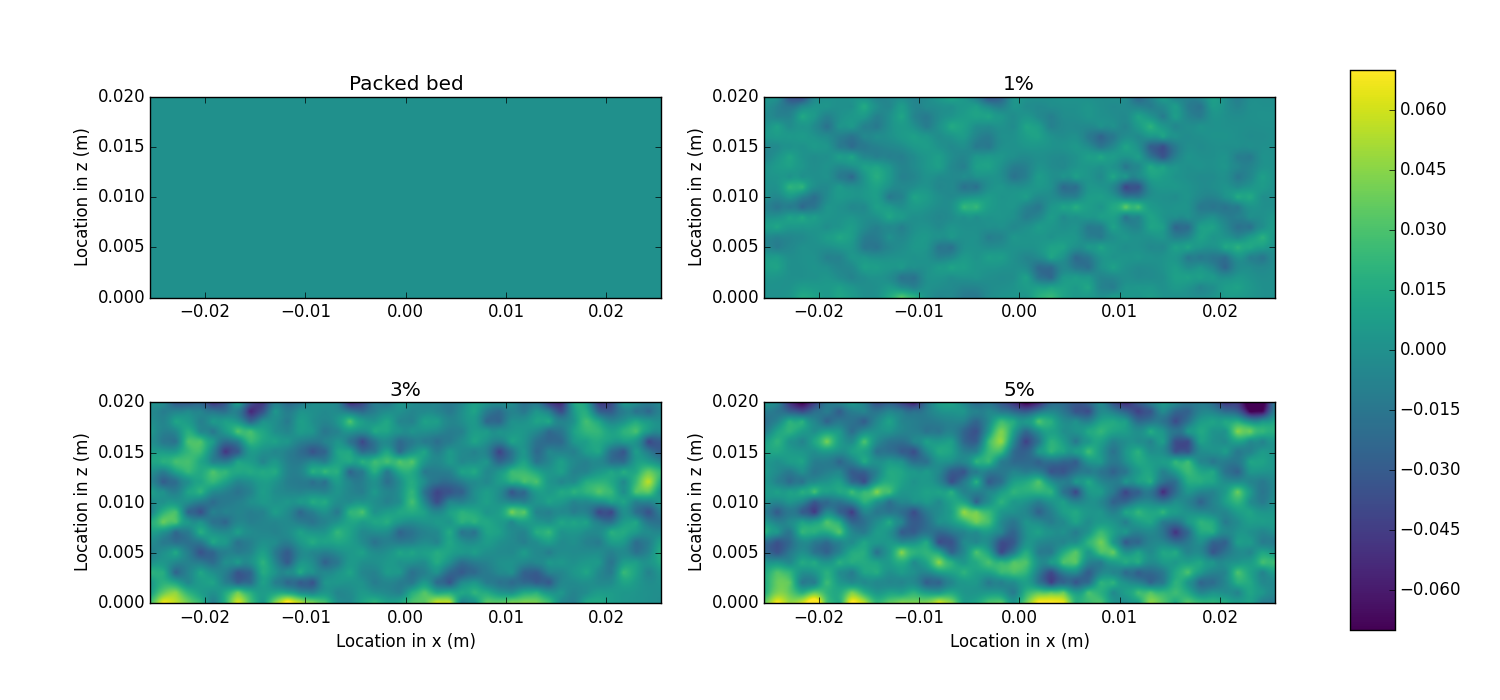
\includegraphics[width = 0.95\textwidth]{figures/z-62-r125-1-deltas.png}
    \caption{Distribution of local changes in packing fraction ($\phi_eta - \phi_i$) for $\zeta$-config, $\phi = 0.64$, $r^* = 0.2$}\label{fig:z-624-r125-deltas}
\end{figure}
% deltas~~~~~~~~~~~~~~~~~~~~~~~~~~


\FloatBarrier

%in each configuration is the near-wall region where pebbles contact walls. In $\chi$-config bed in \Cref{fig:3}, we can see how pebble fragments tumble downward but generally remain in the near-wall region of Zone (1). Conversely, we see clearly in the $\zeta$-config bed of \Cref{fig:1} that some fragment groups leave the region and resettle downward toward the bed's central region. The differences in settling between the two configurations is consistent when we consider pebble behavior in other zones.

%Zones (2) are the moderate temperature regions of \Cref{fig:1,fig:3}, the approximate location is also shown on temperature profiles in \Cref{fig:64-T-profile}. For $\zeta$-configs, temperatures shown in \Cref{fig:64-T-profile} demonstrate an asymmetric lump in profile that is absent in $\chi$-config beds. Increases in Zone (2) temperatures for $\zeta$-config beds are due to the fraction of pebbles which freely tumble through interstitial gaps, influenced by gravity, into Zone (2) from other regions. Once settled, the increased masses of ceramic in Zone (2) then create additional heating from the volumetric source. It should be noted that the exact location of the `lumps' in temperature profiles measured here are unique to the pebble bed considered in this study and the random location at which the fragments accumulated, however the phenomena of increased temperature in the lower-half of $y$-locations of beds with crushed pebbles will consistently appear. As for the $\chi$-configurations, pebbles broken in Zone (2) see their daughter fragments remain in Zone (2) as they tumble in the $y$-direction, regardless of the distance. No added mass in the region results in no abnormal increases in Zone (2) temperature profiles; only overall increases of temperatures are witnessed. 

%For $\zeta$-config beds, a similar effect of fragment-travel into and out of Zone (3) occurs, long-distance traveling of the roughly 10\% of pebbles in $\zeta$ configuration contributes to spreading heat generation from the high temperature regions into regions at lower heights of $y$. However, in $\chi$-config beds, pebbles that crush in Zone (3) again have fragments which generally remain in Zone (3) regardless of distance traveled. The accumulating pebble fragments in Zone (3) continue to receive nuclear heating but have very poor contact conductance with neighboring pebbles. The flowing helium purge gas prevents runaway high temperatures of these fragments but the end results are higher maximum temperatures. In the case of $r_2^*$ at $\eta = 5\%$, we see in \Cref{fig:eta-T_max} the maximum temperatures in $\chi$-config beds overtake the maximum temperatures of similar $\zeta$-config beds. This large increase in maximum temperature rise is due entirely to small fragments accumulation in Zone (3), the similar bed of $\zeta$-configuration shows a much lower maximum bed temperature rise. It is also interesting to note the two beds with smallest temperature rise among any studied here were $\zeta$-configurations. Yet at the same time, those two beds saw similar or more increase in overall bed temperatures in comparison to $\chi$-configurations. These results demonstrate the effect of pebble fragments traveling between zones in $\zeta$-config beds: increasing temperatures in moderate-temperature zones with a trade-off of decreased temperatures in high-temperature zones.

%Looking to \Cref{fig:eta-T_max}, among all the solid lines ($\phi_2 = 0.64$) we see a large jump in bed temperature rise only for the $\chi$-config bed at $\eta = 5\%$ with $r_2^*$; the maximum bed temperature even jumps above most of the less-tightly packed $\phi_1$ beds. It is interesting to note that a similar set of parameters ($\phi_2, r_2^*, \eta_5$) in the $\zeta$-configuration shows a much lower maximum bed temperature rise. Furthermore, 

%, the phenomena of inter-granular resettling strongly impacting temperature rises only occurred for beds with small fragmentation sizes, $r_2^* = 0.2$; see $(\phi_2, \chi_g, r_w^*)$ at $\eta = 5\%$. This is attributed to the tightly packed structures of these well-packed beds. But when the initial packing fraction was reduced, $\phi_1$, for instance, increases in maximum temperatures due to fragment resettling was seen even for larger fragments, $r_1^* =  0.52$. 

%Results shown here illustrate many unique features of heat transfer in granular materials with crushed pebbles and fluid flow. 
%From the temperature profiles of \Cref{fig:T-profiles}, smooth parabolic temperature profiles for initially-packed beds ($\eta = 0$ for both $\phi_{1,2}$) indicate constant $\keff$ values and support the use of continuum theory for those granular assemblies. However, for $\eta > 0$, at all packing fractions and fragmentation radius ratios, temperature profiles become increasingly jagged with large jumps in mean temperatures along $\zeta$ due to heating of crush fragments and distribution of contact forces. Standard models with continuum treatment of granular material cannot predict this manner of inhomogeneous transport of heat in pebble beds. The $\keff$ model must be re-evaluated for use with crushable granular materials.

%for larger crush fragments ($r_1^*$), temperature profiles remained near-perfect parabolas, indicating constant $\keff$ and rough applicability of continuum, for all initial packing fractions and granular crush amounts. However, when fragments were smaller ($r_2^*$), the profiles became more jagged deviation began to occur as crush amount increased. The importance of the profile is in its indication of a constant $\keff$ through the granular material; from the boundary conditions of the system, the more constant the $\keff$, the more perfectly parabolic the temperature profile. This has important repercussions on the the $\keff$ treatment of the granular ceramic as a continuum medium in macro-scale simulations. 

%In \Cref{fig:eta-theta}, total mean temperatures as functions of granular crushing amount are given. Some observable trends: 1) lower initial packing fractions, \textit{i.e.} $\phi_1$, see greater reductions in bed stress and greater mean bed temperatures as pebbles are crushed ; 2) beds with with heat outflow in the direction of gravity ($\zeta$-config) generally had higher bed temperatures for all granular crushing amounts compared to beds with heat outflow perpendicular to gravity ($\chi$-config); 3) size of granular fragment had little impact on bed stresses (until $\eta = 5\%$), but generally beds with smaller fragments had higher temperatures due to small fragments having very small conductive heat transport; 4) when considering fragmentation, there is a weak relationship of internal stress to mean bed temperature. For example, comparing cases of $\phi_2$, $\chi_g$ with the two $r^*_{1,2}$ as functions of $\eta$. For $\eta = 0, 1, 3\%$, stress falls to almost identical values (\Cref{fig:eta-sigma}), yet temperatures for the bed with $r_2^*$ have much higher mean temperatures for all fragmentation amounts.
%If one were to rely only on indirect measurements of pebble bed integrity, \textit{i.e.} measurements of bed pressure load, changes to pebble bed temperature might go unnoticed.

%The polar angle, $\theta$, shown from $0$ to $\pi$ in \Cref{fig:force-polars} is always measured as the angle from $\zeta$ direction -- the mean direction for heat transport to coolant. Thus for all cases, the angles near $\theta = 0,\pi$ correspond to pebbles contacting and transferring heat towards the coolant. Whereas contact between pebbles at angles near $\theta = \pi/2$ correspond to contacts approximately along isotherms in $\chi$ directions (see \Cref{fig:62xpebs}) with little impact on bed heat removal. These plots are more indicative of a pebble bed's ability to transport heat to coolant than bed stresses in \Cref{fig:eta-sigma}. Configurations with $\chi$-direction gravity see higher contact forces near $\theta = 0, \pi$ for all parameters, compared to similar $\zeta$-config beds; likewise the temperatures of $\chi$-config beds are always cooler than similar $\zeta$-config beds. 
%For $\chi$-config cases of \Cref{fig:62-force-polar,fig:64-force-polar}, forces near $\theta = 0,\pi$ are reduced less as individual pebbles are crushed in the ensemble than comparable $\zeta$-config cases. For example, for $\phi_2$, $r^*_1$, mean contact forces near $\theta=0,\pi$ drop by approximately 51\% for $\chi$-configurations whereas mean normal forces drop by nearly 65\% for $\zeta$-configurations. 
%When the internal stress is calculated for pebble beds (for \Cref{fig:eta-sigma}), directional dependence of contact forces is ignored; large forces near $\theta = \pi/2$ mask the reductions in contact forces along heat removal routes. %Therefore overall internal stress of a bed may not drop by a large degree due to large contact forces near $\theta = \pi/2$ directions, but heat transport to boundaries may be strongly affected and temperatures will rise in the bed. 
%This phenomena was observed and mentioned in discussions of \Cref{fig:eta-plots}; and is explainable by directional-dependencies of contact forces and heat transfer in granular systems.


\subsection{Conclusions}
We conducted several multi-scale simulations of granular heat transfer using coupled CFD-DEM simulations of representative tritium-breeding ceramic pebble bed volumes with parametric variations of: bed orientation with respect to gravity, pebble crushing amount, initial packing fraction, and crushed fragmentation size.

There was one general trend observed that reiterates past conclusions from solid breeder research. Namely, more persistent behavior is witnessed in pebble beds with higher initial packing fractions. In this study, the most dominant parameter observed to affect temperatures in pebble beds was the initial packing fraction: beds with higher initial packing fraction had smaller increases in bed temperatures due to pebble crushing. We therefore conclude that manual densification, from either long-term vibration packing or load-induced pre-compaction, must be done to ceramic pebble bed volumes to gain some temperature control during operation in a fusion reactor. To achieve packing fractions of $64\%$ in the relatively small sizes of this study, for example, a load of over \SI{1}{\mega\pascal} was necessary. In the assembly of tritium breeding modules, it must be kept in mind that similar pre-compactions may need to be performed.

As stated earlier, a concern with the $\zeta$ design is the possibility of gap formation between pebble bed and upper walls after bed resettling, particularly after pebble fragmentation. In this study, we found pebble beds initially packed to $\phi = 62\%$ experienced the highest increases in both total average bed temperature as well as maximum temperature rise. The comparably looser packing allowed a quick reduction in bed stresses and consequently a reduction in heat conduction to the upper wall. Nevertheless, no gaps were detected even at 5\% of pebbles crushed. However, temperatures in pebble beds packed to 64\% showed a resistance to fragmentation; overall average temperatures were comparable to $\chi$-configurations, and in fact these EU-style beds had the lowest maximum temperatures for beds with many crushed pebbles. We showed that freedom of fragments to travel between zones in these beds prevented a build-up of loose fragments (and thereby avoided build-up of heating) in the hottest regions.

As for the $\chi$-configurations, we found that when there were not many broken pebbles ($\eta \le 3$\%), these beds generally had lower temperatures in comparison to similar $\zeta$-config beds. But as $\eta$ went above 3\% for many of the beds, the averaged bed temperature and, importantly, the maximum temperature rise actually jumped above the $\zeta$-configurations. We showed that for these beds it was the inability for fragments to move between zones which left many small fragments to settle in the hottest region, further contributing to heating.

From the results we have shown, it is obvious that pebble crushing and bed resettling effects on temperature are complicated, non-linear functions of breeder design and ceramic material employed. We found indications of certain operational spaces for which different designs excelled. For instance, if one were using a material known to have a limited crush strength, one might accept that many pebbles could break (at least up to 5\%, as studied here) over the life of the breeder and choose to employ the $\zeta$-style which avoided large increases in temperature after long operation of the breeder. Alternatively, if one had a ceramic material with a larger crush strength, the $\chi$-design would be preferable as it generally retained lower overall and maximum bed temperatures when fewer pebbles in the ensemble were crushed.

This study was performed on some generic geometries and has provided some generalized conclusions. But in light of the pebble beds' complex responses, as breeder designs continue to evolve into their final form before deployment in ITER, CFD-DEM models should continuously be employed to study the specific thermomechanical responses to pebble crushing and bed resettling unique to each design.


%  We showed that granular crushing in an ensemble resulted in inhomogeneous contact force directional distributions. We also concluded that temperature distributions in beds with granular crushing are not predictable with $\keff$ approximations; demonstrating the limited applicability of continuum modeling of heat transfer in granular material without special consideration for evolving and time-dependent morphologies of the beds. We also discovered that, as pebbles crushed in an ensemble, the effects of structural orientation were reduced in beds with high initial packing fractions. Additionally we found that directional-dependencies of contact forces (\textit{i.e.} magnitudes of contact forces at specific angles of $\theta$) must be considered in situations where there is directional-dependence of heat outflow from bed to coolant.








%%%%%%%%%%%%%%%%%%%%%%%%%%%%%%%%%%%%%%%%%%%%%%%%%%%%%%%%%%%%%%%%%%%%%%%%%%%%%%%%%%%%%%%%%%%%%%
\section{Lattice-Boltzmann Method Modeling of Temperature Distributions in Pebble Beds}\label{sec:lbm-studies}
%3D Lattice-Boltzmann Models of the Complete Conjugate Heat Transfer of Helium Purge Gas and Ceramic Pebble Beds
In this section I apply the relatively new techniques of lattice-Boltzmann method (LBM) numerical modeling to study the complete interstitial flow of helium through a packed bed of lithium ceramics. A discussion on the development of the LBM method was given in \Cref{sec:modeling-lbm}. In that subsection, the advantages of LBM for porous flow simulations were made apparent, namely the potential for extreme parallelization due to the highly local calculations on lattice nodes as well as the straightforward implementation of boundary conditions for the complex geometry of porous networks.

For the implementation of DEM and LBM coupling, pebble packing structures are generated with DEM simulations then mapped into the LBM nodal grids where the thermofluid and conjugate heat transfer models solve momentum and thermal conservation equations. The DEM-LBM approach is a one-way coupled approach in that LBM results are not currently fed back into DEM simulations for future packing evolution. The sacrifice of two-way coupling (that is present in the volume-averaged CFD-DEM model) offers instead to understand the tortuous helium flow and its impact on thermal transport in the tritium breeding ceramic pebble beds.

The first part of this section will discuss the process of determining certain numerical techniques needed in mapping DEM data into LBM nodes. Once the characteristics of the pebble bed parameters are understood, sample models of pebble beds from \Cref{sec:isfnt-12} are loaded into the DEM-LBM solver and analyzed.







\FloatBarrier

\subsection{Model Setup \& Methodology}
The purpose of the lattice-Boltzmann simulation is to reveal the influence of tortuous helium flow on energy transport inside the packed bed of a tritium breeder in a fusion reactor. For this reason, we need not study the same parametric space as that of \Cref{sec:isfnt-12}. Instead we can look at the cases of $\phi = 0.64$ initially packed (with no damage) and then $\phi = 0.64$, $r_2^*$, and $\eta = 5\%$, as described thoroughly in \Cref{sec:isfnt-12}. With a resolution of $\res = 20$, the lattice parameters for both beds are given in \Cref{tab:lbm-parameters}. The relaxation parameters, $\omega$, for the lattice solving the momentum equation ($\omega_{ns}$), the lattice nodes representing the solid in the energy equation ($\omega_{cj}$) and the lattice nodes for the fluid in the energy equation ($\omega_{ad}$) are given in \Cref{tab:lbm-relaxations}

% For this lattice-Boltzmann simulation I use a resolution of $\text{res} = 10$ and a time step of $\delta_t = $\num{0.001}. The rest of the descriptions of our pebble bed are locked from the system and material properties. The other geometric values for the lattice are given in Table~\ref{tab:lbm-parameters}, the relaxation parameters defining the collision dynamics of the lattices are given in Table~\ref{tab:lbm-relaxations}, and the boundary conditions are given in Table~\ref{tab:lbm-boundaries}. The values are all unitless in the lattice framework and are translated from the physical values to match the model of pebbles and fluid from \cref{sec:cfd-dem-studies}

\begin {table}[ht] %
\caption{Physical description of the lattice (in lattice units).}
\label{tab:lbm-parameters} \centering %
\begin {tabular}{ ccccc }
\toprule %
$N_x$   &   $N_y$  &   $N_z$    &   $\delta_x$   & $\delta_t$    \\\toprule
639      &   200     &   50     &    0.1         &  0.001        \\\bottomrule
\end{tabular}
\end{table}

\begin {table}[ht] %
\caption{The momentum relaxation constants for fluid (ns), thermal relaxation constants for fluid (ad), and thermal relaxation constants for the solid (cj) used in the simulation.}
\label{tab:lbm-relaxations} \centering %
\begin {tabular}{ cccccccc }
\toprule %
$\omega_{ns}$ &  $\omega_{ad}$  &   $\omega_{cj}$     \\\toprule
1.132      &  0.988       &   1.365          \\\bottomrule
\end{tabular}
\end{table}

Because we are treating the energy equation as a passive scalar, there is only one-way coupling between the momentum and energy lattices (the Boussinesq approximation is not made for energy-momentum coupling). Furthermore, the fluid flow reaches a steady-state distribution. Therefore, the procedure used here is to first solve only for a steady velocity distribution on the Navier-Stokes lattice. Once steady, the velocity distribution is loaded into the energy lattice and the collision-streaming of the NS lattice does not need to continue. In this way, the long process of reaching thermal steady state can be achieved without the expensive computation of collision-streaming integration of both lattices simultaneously.



% \begin {table}[htp] %
% \caption{Boundary conditions translated into lattice units.}
% \label{tab:lbm-boundaries} \centering %
% \begin {tabular}{ cccccccc }
% \toprule %
% $\vec{u}_\text{inlet}$    &  $T_\text{inlet}$   &  $T_\text{wall}$     \\\toprule
% (0.005, 0, 0)           &  131.79           &   131.79          \\\bottomrule
% \end{tabular}
% \end{table}


% % The physical properties of helium from \cref{sec:cfd-dem-setup} are used here to calculate the relaxation time, $\tau_{ns}$ as outlined in \cref{sec:physical-to-lattice}. The physical description of the pebble bed analyzed with LBM is identical to the beds described in \cref{sec:cfd-dem-studies}. The details for mapping from our DEM packing to the LBM lattice are given in \cref{sec:dem2lbm-mapping}. With the mechanisms described there we can define the lattice nodes definitions (being either solid or fluid) simply with specifying the resolution.

% The relaxation parameter describing the collisions of density distribution functions on the Navier-Stokes lattice (NS-lattice) allowed for achieving a stable and steady fluid velocity. Unfortunately, from the physical properties of ceramic pebbles and thermal properties of helium, the relaxation times on the thermal lattices would only allow the simulation to run until instabilities at the outlet propagates upstream and destroys the results of the entire thermal lattice. These preliminary results will therefore focus on the velocity results and the initial thermal results (it would not reach thermal steady-state before crashing). Even with this caveat on the results, what we do see from the LBM results are extremely encouraging for the use of the method in the future.






% \subsection{Laminar Mixing of Energy in Packed Beds with Volumetric Heating}

% In the plot of \Cref{fig:lbm-streamlines}, streamlines are created along the $y$-direction at the inlet. The streamlines show the inlet helium moving in a tortuous path as it winds through the pebble bed and picks up the energy which has been deposited into the pebbles from a volumetric heat source. The complete tortuous flow field solved in the LBM computations reveals an extremely important feature of the helium purge gas that has, up to now, not been realized.

% Moving up through the $x$ direction of the pebble bed (the direction of the mean flow), several temperature profiles of the fluid and solid are shown in \Cref{fig:lbm-temp-profiles}. The temperature profiles all demonstrate a profile that does not match predicted profiles through pebble beds when constant $\keff$ models are applied to the bed in its continuum treatment. For comparison, the dashed line in \Cref{fig:lbm-temp-profiles} is a parabolic curve with match $\Delta T$ to the profile from $x^* = 10$. 

% Let us explore further the deviation from a parabolic fit and the consequences on solid breeder design that appear from the LBM simulations. In the experimental quantifications of heat transport in pebble beds with interstitial helium, conduction is the only mode of heat transfer considered. The Grashoff number inside a packed bed is small enough that any natural convection cells will most certainly be negligible to heat transfer compared to the conduction through the fluid. Thus, experimentalists can describe the effective thermal conductivity of the combination of solid and gas. These are the values reported in, \textit{e.g.}, \Cref{fig:keff}. The DEM and CFD-DEM studies seemed to support these models as temperature profiles emerged from those simulations that fit nearly perfectly to parabolic profiles of varying $\keff$. Going the other way, if you had a constant $\keff$ of a pebble bed with helium, you could predict temperature profiles, and importantly maximum temperatures, in the solid breeder volume. 

% The $\keff$ value represents the rate at which the solid breeder volume can move energy into the cooling structure. When a perfect parabolic temperature profile is found (such as in the DEM and CFD-DEM results) the $\keff$ is calculated simply from the input volumetric heat source and the $\Delta T$ between centerline and wall. However, because the results from LBM do not fit into a perfect parabolic profile, I fit a parabola of a constant $\keff$ model to the \textit{amount of energy in the profile}. In other words, I integrate the temperature profile from LBM along the $y$ length and find a parabolic profile which, when integrated along the same direction, yields the same value,
% \begin{equation}
%     \int_0^{Y^*} T_{lbm}(y)\,\mathrm{d}y = \int_0^{Y^*} (1-y^2)T_{cl} + T_w y^2
% \end{equation}
% where $T_w$ is the constant temperature wall boundary condition and $T_{cl}$ is the centerline temperature. An iterative procedure is run through until a correct $T_{cl}$ is found which satisfies the equality. When this procedure is carried out, I find the parabola shown in \Cref{fig:lbm-temp-parabolas}.

% Reiterating, the parabola of \Cref{fig:lbm-temp-parabolas} is the shape of temperature profile at which the same amount of energy is removed from the system in a constant $\keff$ condition as is removed from the actual LBM result. What we see in the figure is the LBM result is showing a lower maximum temperature and higher temperature near the walls. This shows that for the amount of energy removed from a pebble bed with flowing helium, the maximum temperature is lower than what would be predicted from current models!

% The phenomena of the flowing helium lowering the maximum temperature in the centerline of the bed and raising the temperature on the edges is something I have given the name of \textit{laminar mixing of energy}. The low Reynolds number flow of helium remains laminar and thus energy transport perpendicular to the flow path of the fluid is still pure conduction. But the tortuous path of helium as it snakes through the pebble bed mixes the energy of hot pebbles in the center and comparatively cooler pebbles near the walls.

% % It is well known that a fluid moving through a packed bed will follow a path much longer than the length of the packed bed. The extended path is often reported as the tortuosity of the packed bed. In the ceramic breeder packed beds for tritium generation, the tortuosity of the helium flow modeled in LB resulted in 

% % \begin{figure}[t]
% %     \centering
% %     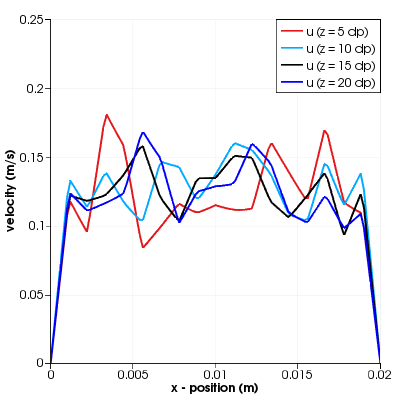
\includegraphics[width=\singleimagewidth]{figures/lbm/evap-u-profiles}
% %     \caption{Velocity profiles (in the $x$-direction) at varying pebble bed heights for the pebble bed with 10\% damaged pebbles.}\label{fig:lbm-evap-u-profile}
% % \end{figure}

% \begin{figure}[t]
%     \centering
%     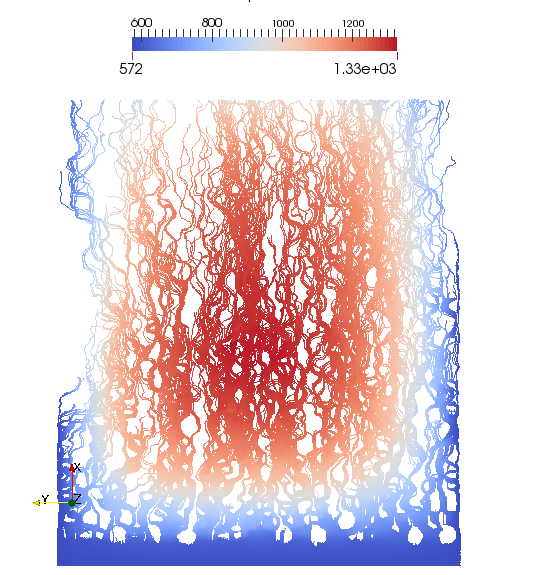
\includegraphics[width=\singleimagewidth]{figures/lbm/lbm-streamlines}
%     \caption{Demonstrating the meandering path -- importantly wandering in the $x$-direction -- of fluid flow in the pebble bed.}\label{fig:lbm-streamlines}
% \end{figure}

% \begin{figure}[t]
%     \centering
%     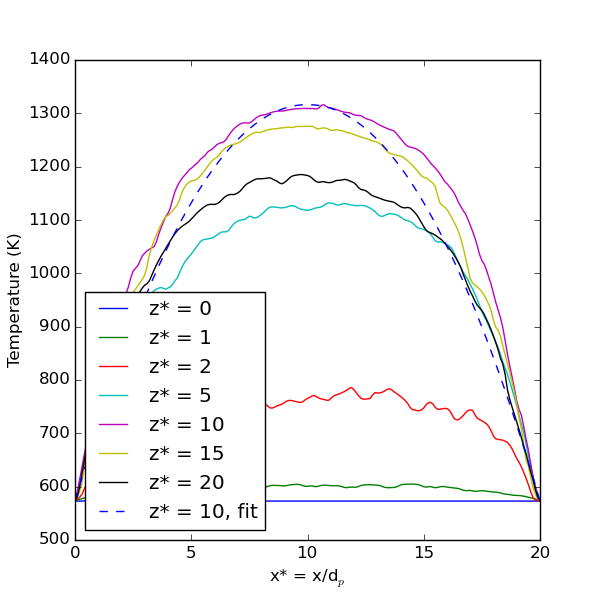
\includegraphics[width=\singleimagewidth]{figures/lbm/lbm-temp-profiles}
%     \caption{Temperature profiles (in the $x$-direction) at varying pebble bed heights for the pebble bed with 10\% damaged pebbles. Shown for comparison is a parabolic profile that had fit both DEM and CFD-DEM temperature results.}\label{fig:lbm-temp-profiles}
% \end{figure}

% \begin{figure}[t]
%     \centering
%     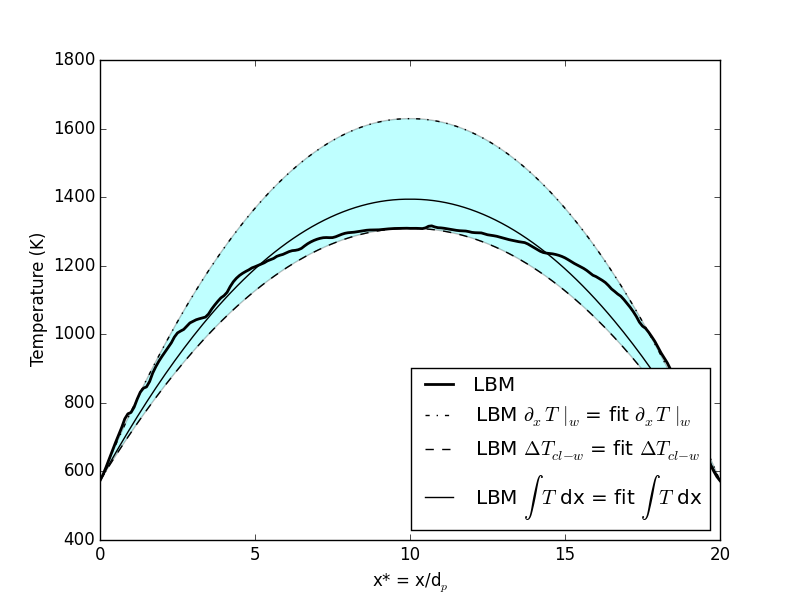
\includegraphics[width=\singleimagewidth]{figures/lbm/lbm-temp-profile_parabolic}
%     \caption{A parabolic fit to the integrated energy of a temperature profile compares to the temperature profile from LBM. The LBM temperature profile increases near the walls and is flattened near the centerline. The behavior is indicative of laminar mixing of energy in the bed.}\label{fig:lbm-temp-parabolas}
% \end{figure}

% \begin{figure}[t]
%     \centering
%     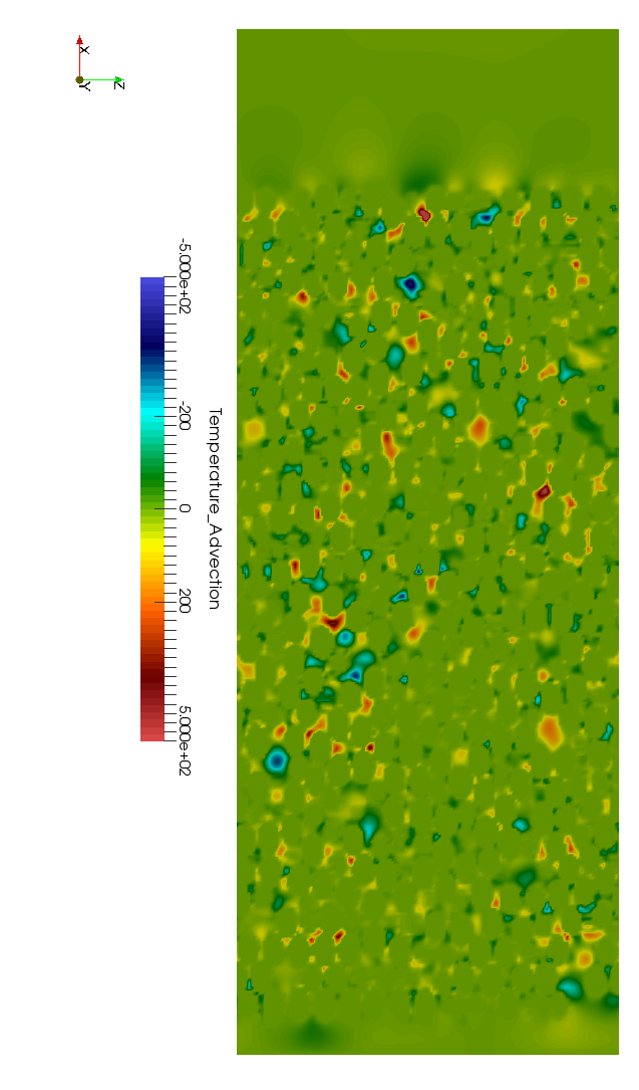
\includegraphics[width=\singleimagewidth]{figures/lbm/lbm-laminar-mixing}
%     \caption{Mean flow direction is in the positive $x$ direction. This $x$-$z$-plane slice shows the $y$ components of velocity as the fluid moves into/out of the plane - mixing the energy with laminar flow.}\label{fig:lbm-laminar-mixing}
% \end{figure}

% \FloatBarrier
% \subsection{Conclusions}




